%
%   Prof. Dr. Julian Reichwald
%   auf Basis einer Vorlage von Prof. Dr. Jörg Baumgart
%   DHBW Mannheim
%
%
%	ACHTUNG: Für das Erstellen des Literaturverzeichnisses wird das modernere Paket biblatex
%			 in Kombination mit biber verwendet -- nicht mehr das ältere BibTex!
% 			 Bitte stellen Sie ggf. Ihre TeX-Umgebung
% 			 entsprechend ein (z.B. TeXStudio: Einstellungen --> Erzeugen --> Standard Bibliographieprogramm: biber)
%

\documentclass[
	12pt,
	BCOR=5mm,
	DIV=12,
	headinclude=on,
	footinclude=off,
	parskip=half,
	bibliography=totoc,
	listof=entryprefix,
	toc=listof,
	pointlessnumbers,
	plainfootsepline]{scrreprt}


%	Konfigurationsdatei einziehen
% !TEX root =  master.tex

%		LANGUAGE SETTINGS AND FONT ENCODING 
%
\usepackage[ngerman]{babel} 	% German language
\usepackage[utf8]{inputenc}
\usepackage{eurosym} % Euro symbol 
\usepackage[german=quotes]{csquotes} 	% correct quotes using \enquote{}
\usepackage[T1]{fontenc}
\usepackage{amssymb} % Mathe-Package
\usepackage{pdfpages} % for appendix pdfs


%\usepackage[english]{babel}   % For english language
%\usepackage{csquotes} 	% Richtiges Setzen der Anführungszeichen mit \enquote{}

% 		HYPERREF
%
\usepackage[
	hidelinks=true % keine roten Markierungen bei Links
]{hyperref}

% Zwei eigene Befehle zum Setzen von Autor und Titel. Ausserdem werden die PDF-Informationen richtig gesetzt.
\newcommand{\TitelDerArbeit}[1]{\def\DerTitelDerArbeit{#1}\hypersetup{pdftitle={#1}}}
\newcommand{\AutorDerArbeit}[1]{\def\DerAutorDerArbeit{#1}\hypersetup{pdfauthor={#1}}}
\newcommand{\Firma}[1]{\def\DerNameDerFirma{#1}}
\newcommand{\Kurs}[1]{\def\DieKursbezeichnung{#1}}


% Correct superscripts 
\usepackage{fnpct}


%		CALCULATIONS
%
\usepackage{calc} % Used for extra space below footsepline



%		BIBLIOGRAPHY SETTINGS
%

% Uncomment the next three lines for author-year-style with footnotes (Chicago)
\usepackage[backend=biber, autocite=footnote, style=authoryear, dashed=false]{biblatex} 	%Use Author-Year-Cites with footnotes
\AdaptNoteOpt\footcite\multfootcite   %will add  separators if footcite is called multiple consecutive times 
\AdaptNoteOpt\autocite\multautocite % will add  separators if autocite is called multiple consecutive times

% Uncomment the next line for IEEE-style 
% \usepackage[backend=biber, autocite=inline, style=ieee]{biblatex} 	% Use IEEE-Style (e.g. [1])

% Uncomment the next line for alphabetic style 
% \usepackage[backend=biber, autocite=inline, style=alphabetic]{biblatex} 	% Use alphabetic style (e.g. [TGK12])

% Uncomment the next two lines vor Harvard-Style 
%\usepackage[backend=biber, style=apa]{biblatex} 	
%\DeclareLanguageMapping{german}{german-apa}


\DefineBibliographyStrings{ngerman}{  %Change u.a. to et al. (german only!)
	andothers = {{et\,al\adddot}},
}

%%% Uncomment the following lines to support hard URL breaks in bibliography 
%\apptocmd{\UrlBreaks}{\do\f\do\m}{}{}
%\setcounter{biburllcpenalty}{9000}% Kleinbuchstaben
%\setcounter{biburlucpenalty}{9000}% Großbuchstaben


\setlength{\bibparsep}{\parskip}		%add some space between biblatex entries in the bibliography
\addbibresource{bibliography.bib}	%Add file bibliography.bib as biblatex resource


%		FOOTNOTES 
%
% Count footnotes over chapters
\usepackage{chngcntr}
\counterwithout{footnote}{chapter}

%	ACRONYMS
%%%
%%% WICHTIG: Installieren Sie das neueste Acronyms-Paket!!!
%%%
\makeatletter
\usepackage[printonlyused]{acronym}
\@ifpackagelater{acronym}{2015/03/20}
  {%
    \renewcommand*{\aclabelfont}[1]{\textbf{\textsf{\acsfont{#1}}}}
  }%
  {%
  }%
\makeatother

%		LISTINGS
\usepackage{listings}	%Format Listings properly
\renewcommand{\lstlistingname}{Quelltext}
\renewcommand{\lstlistlistingname}{Quelltextverzeichnis}
\lstset{numbers=left,
	numberstyle=\tiny,
	captionpos=b,
	basicstyle=\ttfamily\small,
	commentstyle=\itshape,
	breaklines=true, 
	breakatwhitespace=true,
	showstringspaces=false,
	escapeinside={@@},
	keywordstyle=\bfseries,
	postbreak=\raisebox{0ex}[0ex][0ex]{\ensuremath{\hookrightarrow\space}}
	}

%LISTING inline a tabular/table
\newcommand\tablstinline[2][]{\lstinline[#1]{#2}}

% LISTINGS: eigene Programmiersprache; bei morekeywords die zusätzlichen einfügen
\lstdefinelanguage{PLSQL}{
	language     = SQL,
	morekeywords = {over, partition}}

% ---- LISTING FOR YAML FILES ----
%\usepackage[dvipsnames]{xcolor}
%\usepackage{listings}
\usepackage{color}
\newcommand\YAMLcolonstyle{\color{red}\mdseries}
\newcommand\YAMLkeystyle{\color{black}\bfseries}
\newcommand\YAMLvaluestyle{\color{black}\mdseries}

\makeatletter

% here is a macro expanding to the name of the language
% (handy if you decide to change it further down the road)
\newcommand\language@yaml{yaml}

\expandafter\expandafter\expandafter\lstdefinelanguage
\expandafter{\language@yaml}
{
	keywords={true,false,null,y,n},
	keywordstyle=\color{darkgray}\bfseries,
	basicstyle=\YAMLkeystyle,                                 % assuming a key comes first
	sensitive=false,
	comment=[l]{\#},
	morecomment=[s]{/*}{*/},
	commentstyle=\color{purple}\ttfamily,
	stringstyle=\YAMLvaluestyle\ttfamily,
	moredelim=[l][\color{orange}]{\&},
	moredelim=[l][\color{magenta}]{*},
	moredelim=**[il][\YAMLcolonstyle{:}\YAMLvaluestyle]{:},   % switch to value style at :
	morestring=[b]',
	morestring=[b]",
	literate =    {---}{{\ProcessThreeDashes}}3
	{>}{{\textcolor{red}\textgreater}}1     
	{|}{{\textcolor{red}\textbar}}1 
	{\ -\ }{{\mdseries\ -\ }}3,
}

% switch to key style at EOL
\lst@AddToHook{EveryLine}{\ifx\lst@language\language@yaml\YAMLkeystyle\fi}
\makeatother

\newcommand\ProcessThreeDashes{\llap{\color{cyan}\mdseries-{-}-}}
% --------------------------

%		EXTRA PACKAGES
\usepackage{lipsum}    %Blindtext
\usepackage{graphicx} % use various graphics formats
\usepackage[german]{varioref} 	% nicer references \vref
\usepackage{caption}	%better Captions
\usepackage{booktabs} %nicer Tabs
\newcommand{\ra}[1]{\renewcommand{\arraystretch}{#1}}
\usepackage{longtable} %multipages booktabs
\usepackage{array}
%\newcolumntype{P}[1]{>{\raggedright\arraybackslash}p{#1}}


%		ALGORITHMS
\usepackage{algorithm} %float wrapper for algorithms.
\usepackage{algpseudocode}
\renewcommand{\listalgorithmname}{Algorithmenverzeichnis }
\floatname{algorithm}{Algorithmus}


%		FONT SELECTION: Entweder Latin Modern oder Times / Helvetica
\usepackage{lmodern} %Latin modern font
%\usepackage{mathptmx}  %Helvetica / Times New Roman fonts (2 lines)
%\usepackage[scaled=.92]{helvet} %Helvetica / Times New Roman fonts (2 lines)

%		PAGE HEADER / FOOTER
%	    Warning: There are some redefinitions throughout the master.tex-file!  DON'T CHANGE THESE REDEFINITIONS!
\RequirePackage[automark,headsepline,footsepline]{scrpage2}
\pagestyle{scrheadings}
\renewcommand*{\pnumfont}{\upshape\sffamily}
\renewcommand*{\headfont}{\upshape\sffamily}
\renewcommand*{\footfont}{\upshape\sffamily}
\renewcommand{\chaptermarkformat}{}
\RedeclareSectionCommand[beforeskip=0pt]{chapter}
\clearscrheadfoot


\ifoot[\rule{0pt}{\ht\strutbox+\dp\strutbox}DHBW Mannheim]{\rule{0pt}{\ht\strutbox+\dp\strutbox}DHBW Mannheim}
\ofoot[\rule{0pt}{\ht\strutbox+\dp\strutbox}\pagemark]{\rule{0pt}{\ht\strutbox+\dp\strutbox}\pagemark}

\ohead{\headmark}


\begin{document}

%% BITTE GEBEN SIE HIER DEN TITEL UND DIE AUTORIN / DEN AUTOR DER ARBEIT AN!
%% DIESE INFORMATIONEN _MÜSSEN_ GESETZT SEIN, UM TITELBLATT, ABSTRACT UND
%% EIGENSTÄNDIGKEITSERKLÄRUNG AUTOMATISCH ANZUPASSEN!

\TitelDerArbeit{Integration einer Container-Umgebung in einen automatisierten Deployment-Prozess und die Untersuchung ihrer Effekte auf diesen}
\AutorDerArbeit{Yves Torsten Staudenmaier}
\Firma{SV Informatik GmbH}
\Kurs{WWI17SEC}

\begin{titlepage}
\begin{minipage}{\textwidth}
		\vspace{-2cm}
		\noindent 
\includegraphics[scale=0.67]{img/logoeps/SVI-logo-claim.eps} \hfill   
\includegraphics[scale=0.79]{img/logo.jpg}
\end{minipage}
\vspace{1em}
\sffamily
\begin{center}
	\textsf{\large{}Duale Hochschule Baden-W\"urttemberg\\[1.5mm] Mannheim}\\[2em]
	\textsf{\textbf{\Large{}Bachelorthesis}}\\[3mm]
	\textsf{\textbf{\DerTitelDerArbeit}} \\[1.5cm]
	\textsf{\textbf{\Large{}Studiengang Wirtschaftsinformatik}\\[3mm] \textsf{Studienrichtung Software Engineering}}
	
	\vspace{3em}
	\textsf{\Large{Sperrvermerk}}
\vfill

\begin{minipage}{\textwidth}

\begin{tabbing}
	Wissenschaftlicher Betreuer: \hspace{0.85cm}\=\kill
	Verfasser/in: \> \DerAutorDerArbeit \\[1.5mm]
	Matrikelnummer: \> 7146590 \\[1.5mm]
	Firma: \> \DerNameDerFirma  \\[1.5mm]
	Abteilung: \> IE2 -- Deployment \\[1.5mm]
	Kurs: \> \DieKursbezeichnung \\[1.5mm]
	Studiengangsleiter: \> Prof. Dr.-Ing. habil. Dennis Pfisterer \\[1.5mm]
	Wissenschaftlicher Betreuer: \> Marius Ebel \\
	\> info@mariusebel.net \\
	\> +49 176 / 473 45452 \\[1.5mm]
	Firmenbetreuer: \> Thomas Teske \\
	\> thomas.teske@sv-informatik.de \\
	\> +49 621 / 454 44096 \\[1.5mm]
	Lektorat: \> Rita Galli \\[1.5mm]
	Bearbeitungszeitraum: \> 17.02.---08.05.2020
\end{tabbing}
\end{minipage}

\end{center}

\end{titlepage}

\pagenumbering{Roman} % Römische Seitennummerierung
\normalfont

%--------------------------------
% Verzeichnisse - nicht benötige Verzeichnisse bitte auskommentieren / löschen.
%--------------------------------

%   Sperrvermerk
\chapter*{Sperrvermerk}
Der Inhalt dieser Arbeit darf weder als Ganzes noch in Auszügen Personen au"serhalb des Prüfungsprozesses und des Evaluationsverfahrens zugänglich gemacht werden, sofern keine anders lautende Genehmigung der Ausbildungsstätte vorliegt. Die Bachelorarbeit enthält unternehmensinterne Architektur- und Prozessmodellierungen und deren Dokumentation. Es ist zum Zeitpunkt der Anmeldung nicht sicher, ob interne Schnittstellen in der Anwendungslandschaft offengelegt werden.


\vspace{3cm}
\noindent Mannheim, 05.05.2020\hfill\rule{8.4cm}{.4pt}\par
\noindent\hfill Annalena Haus, Ausbildungsverantwortliche
\cleardoublepage



% Lesehinweis
\chapter*{Lesehinweise}
Die folgenden Hinweise sollen das Lesen dieser Projektarbeit erleichtern und spezielle Formatierung definieren:

\begin{itemize}
	\item Im Sinne der Gleichberechtigung wird in dieser Arbeit entweder die Form \textit{\enquote{die Entwickler*in}} oder die grammatikalisch korrekte Form \textit{\enquote{die/der Entwickler/-in}} verwendet werden. Bei der Kurzform mit der Sternnotation wird auf Grund der Lesbarkeit der weibliche Artikel benutzt.
	\item Abbildungen, die mit dem Vermerk \textit{unternehmensintern} gekennzeichnet sind, unterliegen folgendem rechtlichen Hinweis: \enquote{Alle Rechte, einschließlich der Vervielfältigung, Veröffentlichung, Bearbeitung und Übersetzung bleiben der SV Informatik GmbH vorbehalten.}
	\item Produkt- oder Eigennamen werden in \textsc{Kapitälchen} gesetzt, wie beispielsweise \textsc{Node.js}.
	\item Hochgestellte Ziffern weisen auf Fußnoten am Seitenende hin.
	
	
\end{itemize}
 

%	Kurzfassung
\chapter*{Kurzfassung}
\addcontentsline{toc}{chapter}{Abstract}
\begingroup
\begin{table}[h!]
\setlength\tabcolsep{0pt}
\begin{tabular}{p{3.7cm}p{11.7cm}}
Titel: & \DerTitelDerArbeit \\
Verfasser/-in: & \DerAutorDerArbeit \\
Kurs: & \DieKursbezeichnung \\
Ausbildungsstätte: & \DerNameDerFirma\\
\end{tabular}
\end{table}
\endgroup

%Überlege, ob ich den Header brauche mit den ganzen Infos? --> JA.
%Hier können Sie die Kurzfassung der Arbeit schreiben. 
Kurze Einleitung: Motivation, Einführung in den Themenkomplex, allgemeine Methodik
\par
Forschungsfrage eins: Frage + kurze Erläuterung - Methodik - Teil-Ergebnis
\par
Forschungsfrage zwei: Frage + kurze Erläuterung- Methodik - Teil-Ergebnis
\par
Forschungsfrage drei: Frage + kurze Erläuterung - Methodik - Teil-Ergebnis
\par
Minimalergebnis

%	Inhaltsverzeichnis
\tableofcontents

%	Abbildungsverzeichnis
\listoffigures 

%	Tabellenverzeichnis
\listoftables

%	Listingsverzeichnis
\lstlistoflistings
 

% 	Algorithmenverzeichnis
%\listofalgorithms

% 	Abkürzungsverzeichnis (siehe Datei acronyms.tex!)
\clearpage
\chapter*{Abkürzungsverzeichnis}	
\addcontentsline{toc}{chapter}{Abkürzungsverzeichnis}


\begin{acronym}[RDBMS]
	\acro{AWL}{Anwendungslandschaft}
	\acro{DHBW}{Dualen Hochschule Baden-Württemberg}
	\acro{BaFin}{Bundesanstalt für Finanzdienstleistungsaufsicht}
	\acro{IE2}{IE2 -- Deployment}
	\acro{IE}{IE -- Entwicklungs- und Betriebsunterstützung}
	\acro{CAB}{\enquote{Change Advisory Board}}
	\acro{ITIL}{Information Technology Infrastructure Library}
	\acro{SV}{SV SparkassenVersicherung}
	\acro{SVI}{SV Informatik GmbH}
	\acro{SVS}{SV Sachsen}

\end{acronym}

\ohead{Acronyms} % Neue Header-Definition

%--------------------------------
% Start des Textteils der Arbeit
%--------------------------------
\clearpage
\ihead{\chaptername~\thechapter} % Neue Header-Definition (inner header)
\ohead{\headmark} % Neue Header-Definition (outer header)
\pagenumbering{arabic}  % Arabische Seitenzahlen

%	Anleitungs-Datei anleitung.tex einziehen. Auf diese Weise sollten Sie versuchen, für jedes einzelne
% Kapitel eine eigene Datei anzulegen und mittels input-Kommando einzuziehen.
%\input{anleitung}

%-----------------
% Kapitel einbinden
%-----------------

% reset memory of all acronyms, so \ac will print out full name of acronym!
\acresetall 
\hyphenation{An-wendungs-land-schaft} % because ngerman/babel doesn´t know it correctly... 

\chapter{Einleitung}\label{kap:einleitung}
\paragraph{Motivation der Arbeit}
Die \ac{SV} ist bestrebt ihre Versicherungsprozesse und den Kontakt mit den Kunden durch digitale Kanäle ständig zu verbessern. Die Digitalisierung ist ein wichtiger Bestandteil der \ac{SV}-Strategie: So ist sie Mitbegründerin der \enquote{id-fabrik}\footnote{Ein Start-up, das federführend Innovationen im Bereich der S-Finanzgruppe erzeugt.} und Mitglied im \enquote{InsurLab Germany}\autocite[vgl.][S.\,30]{sv_sparkassenversicherung_sv_2019}. Um die Anforderungen der \ac{SV}-Kunden nach ständiger Verfügbarkeit und hoher Servicequalität zu erfüllen, muss die \ac{SV} ihre \ac{AWL} ständig an diese Anforderungen anpassen. Die Nachfrage der \ac{SV}-Kunden und damit die daraus resultierenden Anforderungen an die Systeme, stellt die IT-Dienstleisterin (\ac{SVI}) der \ac{SV} vor neue Herausforderungen. Die Verteilungsprozesse von neuen Versionen der Anwendungen können derzeit nicht während des laufenden Betriebes durchgeführt werden. So müssen neue Funktionen warten, bis das Wochenende des \enquote{Release} sie veröffentlicht, d.\,h. die \ac{TTM} der neuen Produkte ist sehr hoch. Diese Verzögerung der Produktveröffentlichung passt nicht zu der digitalen Strategiezielen der \ac{SV}. Als Lösungsansatz sind die Eigenschaften der \enquote{Cloud}-Technologie zu nennen. Jedoch muss aus IT-Sicht hier eine Anmerkung gemacht werden:

\begin{figure}[h!]
	\centering
	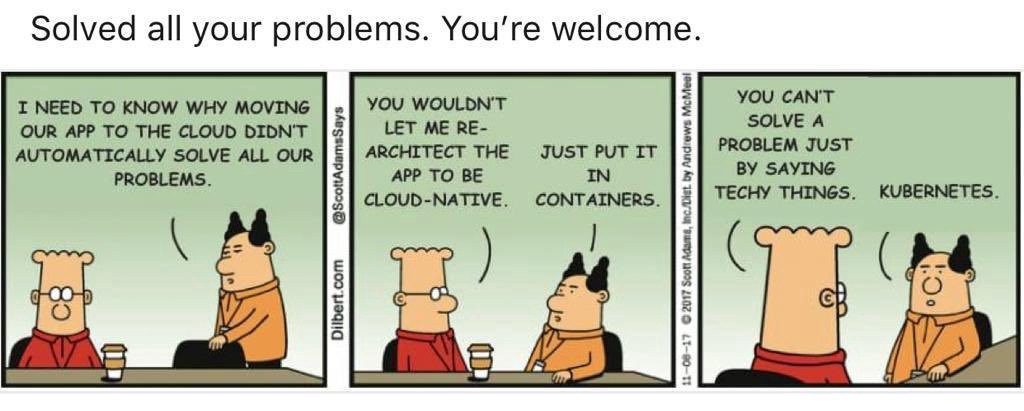
\includegraphics[scale=0.33]{img/dilbertCloud.jpeg}
	\caption{Dilbert-Comic zu \textsc{Kubernetes}}
	\label{abb:dilbertK8s}
	{\footnotesize Quelle: \cite{DilbertKubernetes}\par}
	{\footnotesize Redaktionelle Anmerkung: Abbildung nur als komprimiertes Format verfügbar (Qualitätseinbuße)}
\end{figure}

Die, in Abbildung \vref{abb:dilbertK8s}, dargestellte Aussage ist absichtlich überspitzt, um das Verständnis der Lösungsmöglichkeiten der \enquote{Cloud}-Technologie zu schärfen. Der Hinweis der IT stellt klar, dass das oben beschriebene Problem nur mit einer ganzheitlichen Lösung zu erreichen ist. Es führt nicht zum gewünschten Ergebnis, Anwendungen, die nicht für die \enquote{Cloud} gedacht sind, mit Zwang in diese zu bewegen. Diese Arbeit beschreibt den Prozess zur Verteilung von Container-Anwendungen. 

\paragraph{Problemstellung und -abgrenzung}
Bei der vorliegenden Arbeit handelt es sich um eine mehrteilige Analyse und Konzeption, die bei abgeschlossener Untersuchung ein Konzept zur automatischen Verteilung von Container-Anwendungen, die Betrachtung der Effekte von diesen Anwendungen und ein Ergebnis zu den sicherheitsrelevanten Aspekten dieses Prozess enthalten wird. Dabei akkumuliert sich der Fokus die Prozessentwicklung der Verteilung einer Container-Anwendung. Des Weiteren ist die Untersuchung der Anforderungen, die Analyse der \enquote{Cloud}-Plattform \textsc{OpenShift}\footnote{\enquote{\textsc{OpenShift} is an open source container application platform by Red Hat based on the Kubernetes container orchestrator for enterprise app development and deployment.} Quelle: \cite[][]{red_hat_inc_openshift_2020}} und die Erstellung eines Generierungsalgorithmus im Fokus dieser Arbeit. Dieser Teilkomplex wird durch die Forschungsfrage eins -- Wie können Container-Anwendungen den Prozess des automatisierten \enquote{Deployments}\footnote{\enquote{Software deployment may be considered to be a process consisting of a number of inter-related activities including the release of software at the end of the development cycle; the configuration of the software, the installation of software into the execution environment, and the activation of the software. It also includes post installation activities including the monitoring, deactivation, updating, reconfiguration, adaptation, redeploying and undeploying of the software.} (\cite{dearle_software_2007})} unterstützen? -- abgedeckt. Der Anforderungskatalog soll in Zusammenarbeit mit dem Fachbereich erstellt werden, um die Akzeptanz der Anforderungen zu steigern und um die Validität dieser zu gewährleisten. Die Forschungsfragen zwei und drei (siehe dazu Paragraph \enquote{Forschungsfragen/-design}) analysieren den wirtschaftlichen und sicherheits-/rechtlich-relevanten Bereich des Themenkomplexes der Bachelorarbeit. Dabei bedient sich die Forschungsfrage zwei der Methodik des Geschäftsvorfalls (\enquote{Business Case}). Beide Forschungsfragen werden durch eine Analyse des Ist-Zustands eine initiale Konzeption ableiten. 
\par
Nicht Teil dieser Arbeit ist die unternehmensinterne Entscheidung über die Verantwortlichkeiten des zu entwickelnden Prozesses und die Erstellung einer unternehmensweiten Strategie zum Container-\enquote{Deployment}. Die Anpassung des unternehmensinternen Prozesses \enquote{Release} ist nicht Teil dieser Arbeit. Dieser übersteigt die Anforderungen, die an diese Bachelorarbeit gestellt werden. Auch genügt die rechtliche Betrachtung des Einkaufsprozess von Software nicht den juristischen Ansprüchen eines Gutachtens. Dies ist jedoch nicht Ziel der Arbeit. Die wirtschaftliche Betrachtung des Geschäftsvorfalls  \enquote{Container-Verteilung} dient als reine Veranschaulichung der Methodik und genügt nicht einer vollständigen Betrachtung, die die \ac{BWL} vorgibt. Der Fokus der Arbeit liegt auf der technischen Entwicklung eines Verteilungsprozesses.

\paragraph{Zielstellung der Arbeit}\label{kap:einleitung:Ziele}
Folgende \textit{SMART}\footnote{\enquote{SMART-Regel sind Formulierungshilfen, die eine einfache Methode zum Operationalisieren von Zielen und auch zur Überprüfung der Güte von Zielen darstellen.} Quelle: \cite[][S.69]{dechange_projektmanagement_2020}} formulierte Ziele sollen diese Bachelorthesis leiten, messbar machen und später als Anhaltspunkt zur Evaluierung des Erfolgs dienen:

\begin{enumerate}
	\item Entwicklung eines Verteilungsprozess für einfache Container-Anwendungen bis zum 27.April 2020. Einfach bedeutet hier, dass die Container-Struktur aus einer \enquote{Base Image}\footnote{siehe dazu Kapitel \vref{kap:container}}-Schicht und einer Logik-Schnitt (Eigenentwicklung) besteht.
	\item Der Prozess muss zu 98\,\% ohne Einwirkung von Menschen während des Verteilungsvorgangs funktionieren, d.\,h. er ist (annähernd) voll automatisiert. Dies muss bis zum Ende des Bearbeitungszeitraum der Arbeit (8.Mai 2020) umgesetzt werden.
	\item Die Generierung einer Konfigurationsdatei soll in 9 von 10 Verteilungen automatisch mit einem Skript durchgeführt werden. Umzusetzen ist dies bis zum 08.Mai 2020.
	\item Die Vorteile einer Container-Anwendung für die Verteilung dieser sollen erforscht werden. Akzeptiert ist dieses Ziel, sobald eine Auflistung und eine kritische Betrachtung der Ergebnisse beschrieben wurde. Umzusetzen bis zum Ende des Bearbeitungszeitraums. (Dieses Ziel ist nicht komplett \textit{SMART}-konform, da die zumindest die Messbarkeit ohne genannte Messgröße nicht nachvollziehbar ist.)
	\item Die wirtschaftliche Betrachtung muss sich anhand des Standes von Wissenschaft und Technik orientieren. Dazu werden gängige Regeln von \cite{herman_is_2009}, \cite{brugger_it_2009} u.\,Ä. benutzt. Diese Betrachtung muss bis zum Ende des Bearbeitungszeitraums durchgeführt werden. Die Messbarkeit wird durch die Einhaltung der oben genannten Regeln beschrieben.
	\item Die sicherheits-/rechtlich-relevanten Aspekte dieses Projektes sollen anhand der, für die Finanzdienstleitungs- und Versicherungsbranche, geltenden Vorschriften beleuchtet werden. Der Umfang dieser Beleuchtung beschränkt sich auf das Nötigste, d.\,h. es müssen nur die wichtigsten Regeln beschrieben werden. Dies ist bis zum Ende des Bearbeitungszeitraumes umzusetzen. Die Messbarkeit ist durch die sicherheits-/rechtlich-relevanten Vorschriften bestimmt.
\end{enumerate}

\paragraph{Forschungsfragen/-design}\label{ffs}
Die Forschungsfragen, mit der sich diese Bachelorarbeit beschäftigen wird, sind eine direkte Konsequenz aus der Zielstellung der Arbeit und aus den unternehmensinternen Anforderungen an eines möglichst vollständig automatisierten Prozesses. Dabei liegt der Fokus auf der Betrachtung beider Teildisziplinen der Wirtschaftsinformatik, nämlich der Informatik und der Wirtschaft -- jedoch wird der größere Teil dieser Arbeit einen informationstechnischen Fokus haben. Die folgende Aufzählung nennt die einzelnen Forschungsfragen, die im weiteren Verlauf ein gemeinsames Ergebnis erbringen werden. Dieses ist in Kapitel \vref{kritischeBetrachtung} dargestellt.
\begin{enumerate}
	\item Wie können Container-Anwendungen den Prozess des automatisierten \enquote{Deployments} unterstützen?
	\item Welche wirtschaftlichen Vorteile hat der Einsatz von Containern auf den Prozess des automatisierten \enquote{Deployments}?
	\item Welche besonderen sicherheitstechnischen Aspekte muss ein solcher Prozess im Bereich der Versicherung erfüllen?
\end{enumerate}
% TODO: Nachfolgende Absätze auf Richtigkeit prüfen
Die Forschungsfrage eins wird einen Ist-Zustand analysieren. Diese Analyse enthält eine Betrachtung des Prozesses und einen Anforderungskatalog der Entwicklungsabteilungen an den zu konzeptionierenden \enquote{Deployment}-Prozess für Container-Anwendungen. Danach wird ein Konzept eines Container-basierten automatisierten \enquote{Deployment}-Prozesses erstellt, das aus der Entwicklung dieses und einer Standardisierung der beteiligten Dateien besteht. Die Forschungsfrage eins schließt mit einem Teilergebnis ab. \par

Die Forschungsfrage zwei beschäftigt sich mit den wirtschaftlichen Vorteil eines Einsatzes der Container auf den Prozess des automatisierten \enquote{Deployment}-Prozesses. Dabei wird der bestehende Geschäftsprozess \enquote{Release} analysiert und ein Ist-Soll-Vergleich der Methodik des \enquote{Business case} mit der Umsetzung im Unternehmen durchgeführt. Ein Ausblick schließt die Forschungsfrage zwei ab. 
\par
Die Forschungsfrage drei identifiziert sicherheitsrelevante Anforderungen, die nicht nur die Anwendung selbst betreffen, sondern Auswirkung auf die komplette Anwendungslandschaft (\acs{AWL}) haben. Diese Anforderungen werden durch das \acl{BSI} und verschiedene \textsc{DIN/ISO}-Normen beeinflusst. Außerdem soll analysiert werden, wie bei der Beschaffung von \enquote{Open source}- bzw. \enquote{Closed source}-Anwendungen mögliche Schwachstellen identifiziert werden, die potenzielle Angriffsvektoren in der \ac{AWL} eröffnen würden, und wie mit diesen verfahren wird. Dabei soll versucht werden Rückschlüsse auf die Anwendung \textsc{OpenShift} von \textsc{Red Hat\footnote{\enquote{Red Hat ist der weltweit führende Anbieter von Open-Source-Lösungen, die auf verlässlichen und leistungsstarken Technologien in den Bereichen \enquote{Cloud}, Virtualisierung, Storage, Linux, Mobile und Middleware basieren. Darüber hinaus bieten wir Support-, Trainings- und Consulting-Services an, die mehrfach prämiert wurden.} Quelle: \cite[][]{red_hat_inc_red_2020}}} zu ziehen. Auch hier wird ein Teilergebnis diese Forschungsfrage abschließen


\paragraph{Einordnung der Abteilung in den Geschäftsprozess}
Die Abteilung \ac{IE2}, die aus Sicht des unternehmensinternen Organigramms der Organisationseinheit \ac{IE} angehört, befasst sich in erster Linie mit dem Transport (\enquote{Deployment}) von Software-Artefakten der einzelnen Software-Produkte der \ac{SVI}. Diese werden für die \ac{SV} entwickelt, betrieben und gewartet. Zu den zentralen Aufgaben der Abteilung gehören die Planung, die Durchführung und die Überwachung der \enquote{Build/Deployment}-Prozesse der verschiedenen Service-Umgebungen, die aus mehreren Server-Verbünden bestehen. Des Weiteren stellt \ac{IE2} die Einspielung von datenbank-relevanten Objekten sicher. Auch entwickelt sie die Bau- und Transportprozesse kontinuierlich weiter und passt diese an die sich ständig verändernden Anforderungen der Entwicklungsabteilungen an. Von zentraler Bedeutung sind die Planung und die Durchführung der Veröffentlichungen der neuen Versionen einer zu betreuenden Anwendung. Zu dieser Aufgabe gehören auch Aufbau und Bereitstellung der Systemtest-, Releasetest- und Produktionsumgebungen. Eine weitere zentrale Aufgabe ist das Umgebungsmanagement. Die Aufgaben dieses Teilbereichs befassen sich mit folgenden Inhalten: Planung von Aktivitäten in der Produktionsumgebung, der Planung und der Koordination der Infrastruktur und Notfall-\enquote{Fix} der Produktion und der allgemeinen \enquote{Patch}-Planung; Beratung zur Erweiterung, Koordination und Planung von verschiedenen Testumgebungen. Außerdem ist das Umgebungsmanagement Teil des \ac{CAB}, das ein Gremium nach der \enquote{Best practice} \ac{ITIL} darstellt. Dieses ist für die Freigabe von \enquote{Changes} verantwortlich und hat sowohl ständige, als auch der Situation angepasste Mitglieder. 

\paragraph{Aufbau der Arbeit}
In Kapitel \vref{ff1} wird die Forschungsfrage eins behandelt. Diese beschreibt grundlegende Aspekte der Anforderungsanalyse, des \acl{Cloud-C} und der Container(-isierung)/Orchestrierung. Diese Grundlagen werden später benutzt, um das Vorgehen in diesem Kapitel nachvollziehbar zu gestalten. Die Anforderungsanalyse erkundet die Wünsche der Fachbereiche im Bezug auf die Verteilung von Container-Anwendungen und entwickelt daraus Anforderungen, die dem Stand der Wissenschaft genügen. Wichtig in diesem Kapitel ist die Entwicklung des Prozesses und die damit verbundene Beschreibung der Tätigkeiten.
\par
In Kapitel \vref{ff2} wird die Forschungsfrage zwei behandelt:
\par
In Kapitel \vref{ff3} wird die Forschungsfrage drei behandelt: 
\par
In Kapitel \vref{kritischeBetrachtung} 


%-----------------

\clearpage
\pagenumbering{Roman}
\setcounter{page}{10} %TODO: schauen, ob die "9" passt.

%	Literaturverzeichnis
\printbibliography[title=Literaturverzeichnis]
\cleardoublepage

% Der Anhang beginnt hier - jedes Kapitel wird alphabetisch aufgezählt. (Anhang A, B usw.)
\appendix
\ihead{\appendixname~\thechapter} % Neue Header-Definition

% appendix.tex einziehen
\addcontentsline{toc}{chapter}{Anhang} %sorgt für eintrag ins inhaltsverzeichnis
\chapter{Ergänzungen zur Forschungsfrage eins} \label{appendixFF1}
In diesem Teil des Anhangs sind Ergänzungen zur Forschungsfrage eins des Kapitels \vref{ff1} beschrieben.

\section{Anforderungsdokument}\label{appendixAnforderung}

Ein Anforderungskatalog hat bestimmte Anforderungen, die an den Katalog gestellt werden. Neben der Forderung nach Einhaltung der Qualitätskriterien, definiert nach dem ISO-Standard 9000/9001, sind noch folgende Forderungen in der Literatur beschrieben: \autocite[sig.][S.34]{partsch_requirements-engineering_2010}

\begin{itemize}
	\item vollständig (inhaltlich – d. h., alle Anforderungen sind erfasst –, formal, Norm-konform)
	\item konsistent (keine Widersprüche zwischen den Bestandteilen des Dokuments,
	insbesondere keine Konflikte zwischen verschiedenen Anforderungen)
	\item lokal änderbar (Änderungen an einer Stelle sollten keine Einflüsse auf Konsistenz und Vollständigkeit des Gesamtdokuments haben)
	\item verfolgbar (ursprüngliche Stakeholderwünsche und Zusammenhänge zwischen
	Anforderungen sind leicht zu finden)
	\item klar strukturiert
	\item umfangsmäßig angemessen
	\item sortierbar/projizierbar (nach verschiedenen Kriterien, für verschiedene Stakeholder).
\end{itemize}

Die folgende Aufzählung beschreibt eine Vorlage für das Anforderungsdokument nach Quelle: Sie nutzt die Hilfsmittelsammlung \enquote{Volere}. Diese bietet im Themenbereich \enquote{requirements engineering} kostenpflichtig Dokumentenvorlagen an. Die beiden Bekanntesten sind die hier gezeigte \enquote{Volere Requirements Specification Template} und das kostenlose \enquote{Volere Atomic Requirement Template}, das umgangssprachlich \enquote{Snow Card} genannt wird. Die \enquote{Snow Card} (\vref{abb:volereSnowCard}) ist eine Karteikarte, die benutzt wird, um eine vollständige Aufnahme aller Informationen einer einzelnen Anforderung zu gewährleisten.\autocite[vgl.][]{VolereSnowCard} 

\begin{figure}[H]
	\centering
	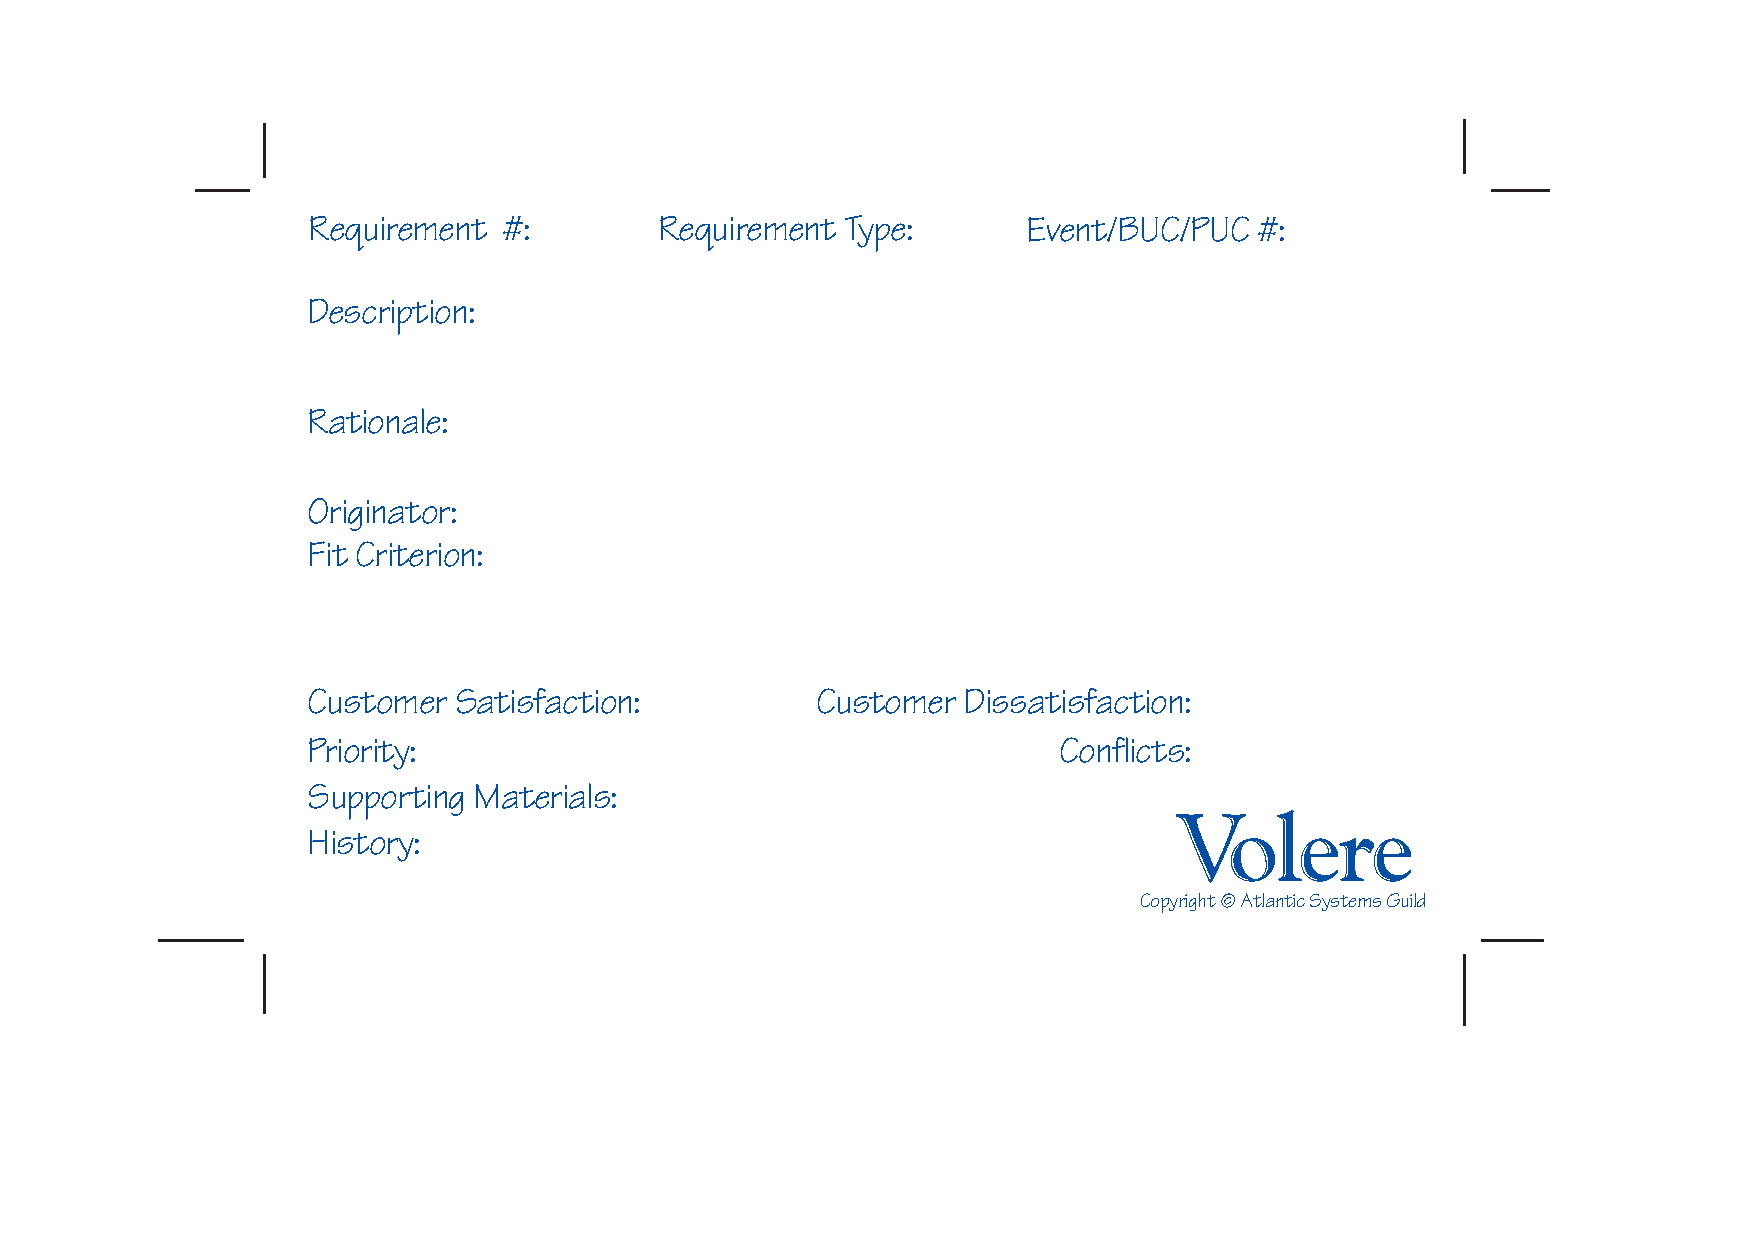
\includegraphics[scale=0.6]{img/snowcard.pdf}
	\caption{Volere Snow Card}
	{\footnotesize Quelle: \cite{VolereSnowCard}}
	\label{abb:volereSnowCard}
	%		{\scriptsize \textit{Alle Rechte, einschließlich der Vervielfältigung, Veröffentlichung, Bearbeitung und Übersetzung bleiben der SV Informatik GmbH vorbehalten.}}
\end{figure}

Die folgende Liste wurde in Anlehnung an die Quelle \cite{VolereRequirmentsSpecTemplate} erstellt.

\begin{minipage}{\linewidth}
	\begin{itemize}\label{abb:volereReqSpec}
		\item Projekt-Treiber
		\begin{enumerate}
			\item Zweck des Projekts
			\item Auftraggeber, Kunde und andere Stakeholder
			\item Nutzer des Produkts
		\end{enumerate}
		\item Projekt-Randbedingungen
		\begin{enumerate}
			\item Einschränkungen
			\item Namenskonventionen und Definitionen
			\item Relevante Fakten und Annahmen
		\end{enumerate}
		\item Funktionale Anforderungen
		\begin{enumerate}
			\item Arbeitsrahmen
			\item Systemgrenzen
			\item Funktionale und Daten-Anforderungen
		\end{enumerate}
		\item Nicht-funktionale Anforderungen
		\begin{enumerate}
			\item Look-and-Feel-Anforderungen
			\item Usability-Anforderungen
			\item Performanz-Anforderungen
			\item Operationale und Umfeld-Anforderungen
			\item Wartungs- und Unterstützungsanforderungen
			\item Sicherheitsanforderungen
			\item Kulturelle und politische Anforderungen
			\item Rechtliche Anforderungen
		\end{enumerate}
		\item Projekt-Aspekte
		\begin{enumerate}
			\item Offene Punkte
			\item Standardlösungen
			\item Neu aufgetretene Probleme
			\item Installationsaufgaben
			\item Migrationstätigkeiten
			\item Risiken
			\item Kosten
			\item Nutzerdokumentation
			\item Zurückgestellte Anforderungen
			\item Lösungsideen
		\end{enumerate}
	\end{itemize}
\end{minipage}

\clearpage
\begin{figure}[H]
	\centering
	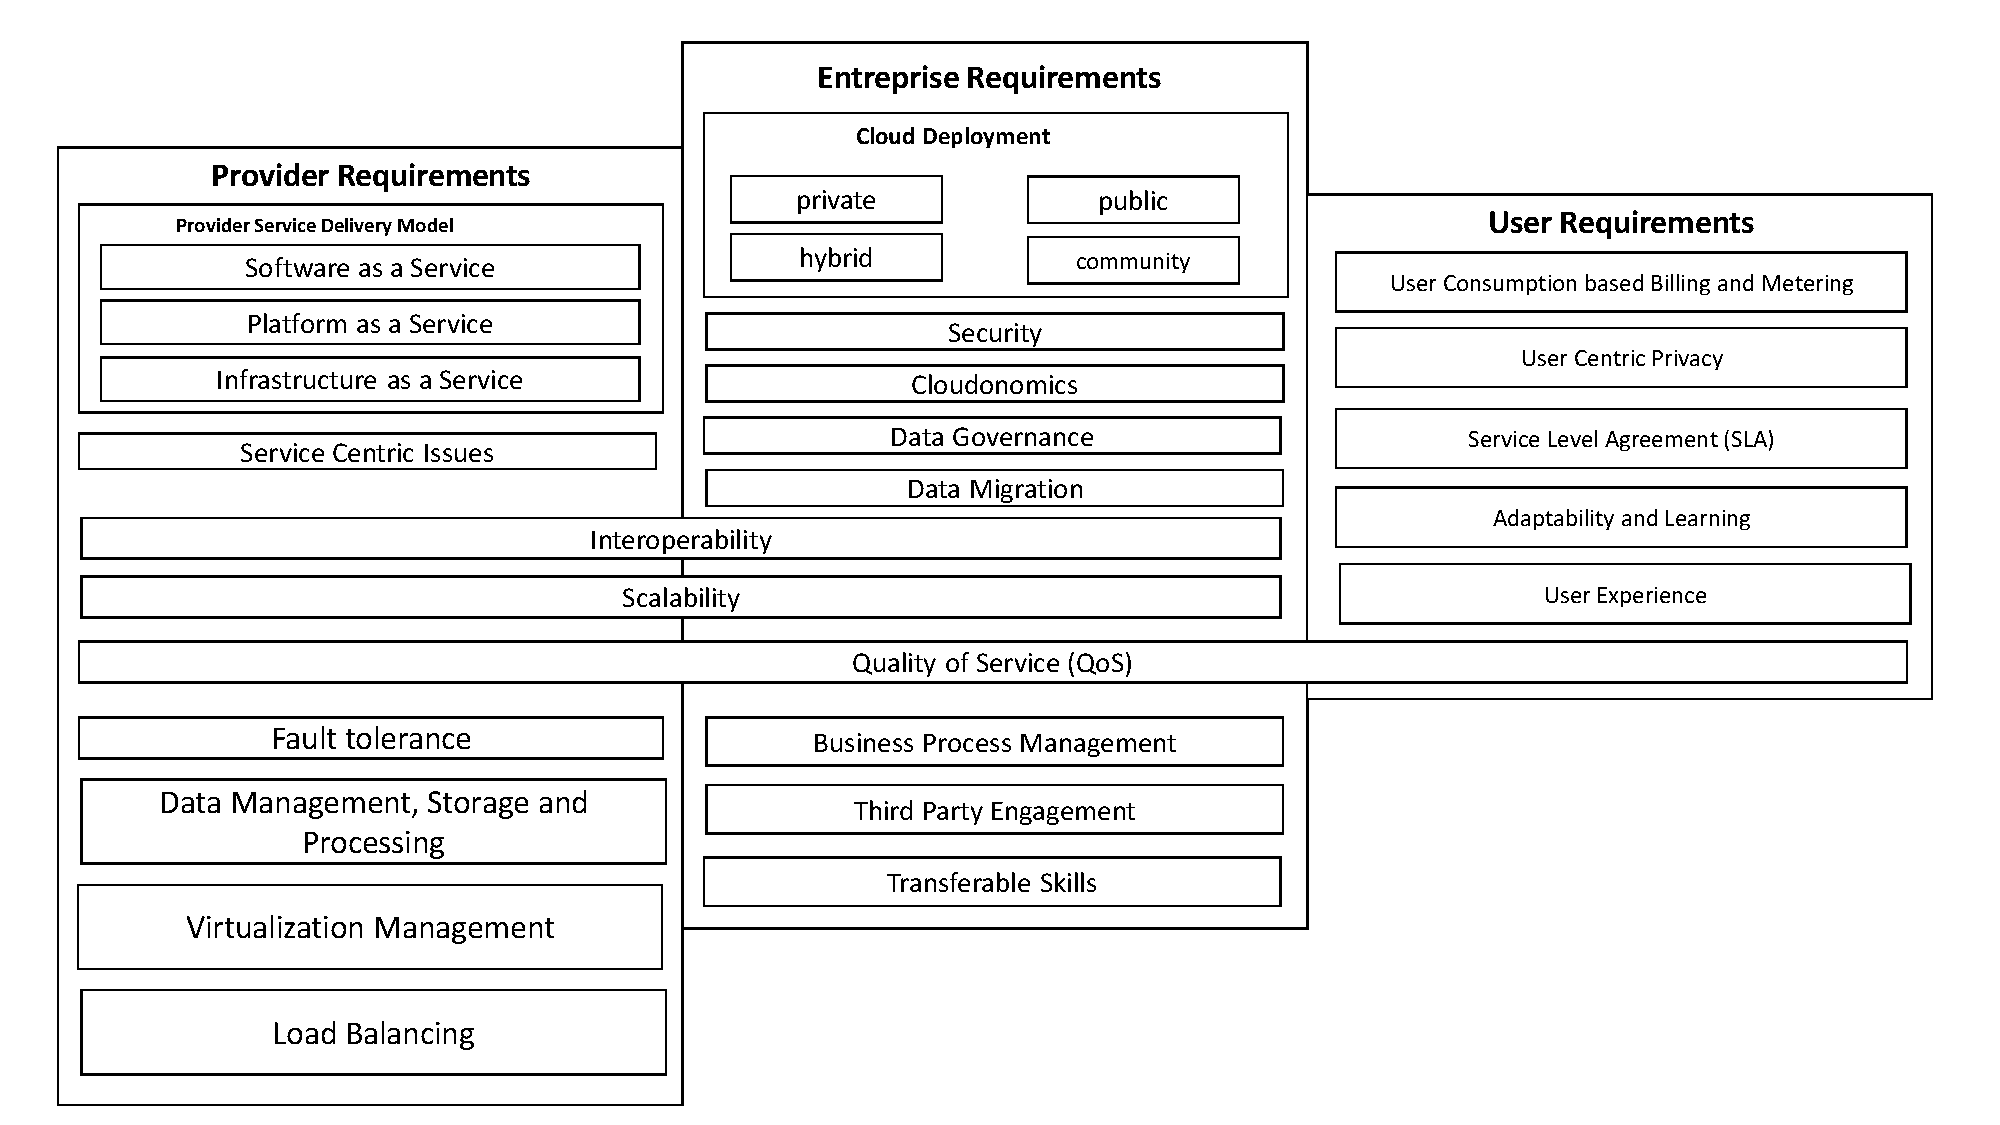
\includegraphics[scale=0.50, angle=90]{img/cloudreq.pdf}
	\caption{Ebenen der \enquote{Cloud}-Anforderungsanalyse}
	{\footnotesize Quelle: in Anlehnung an \cite{rimal_architectural_2011}}
	\label{abb:cloudreq}
	%		{\scriptsize \textit{Alle Rechte, einschließlich der Vervielfältigung, Veröffentlichung, Bearbeitung und Übersetzung bleiben der SV Informatik GmbH vorbehalten.}}
\end{figure}

\clearpage
\section{Statistiken zum Themengebiet \ac{Cloud-C}}

\begin{figure}[H]
	\centering
	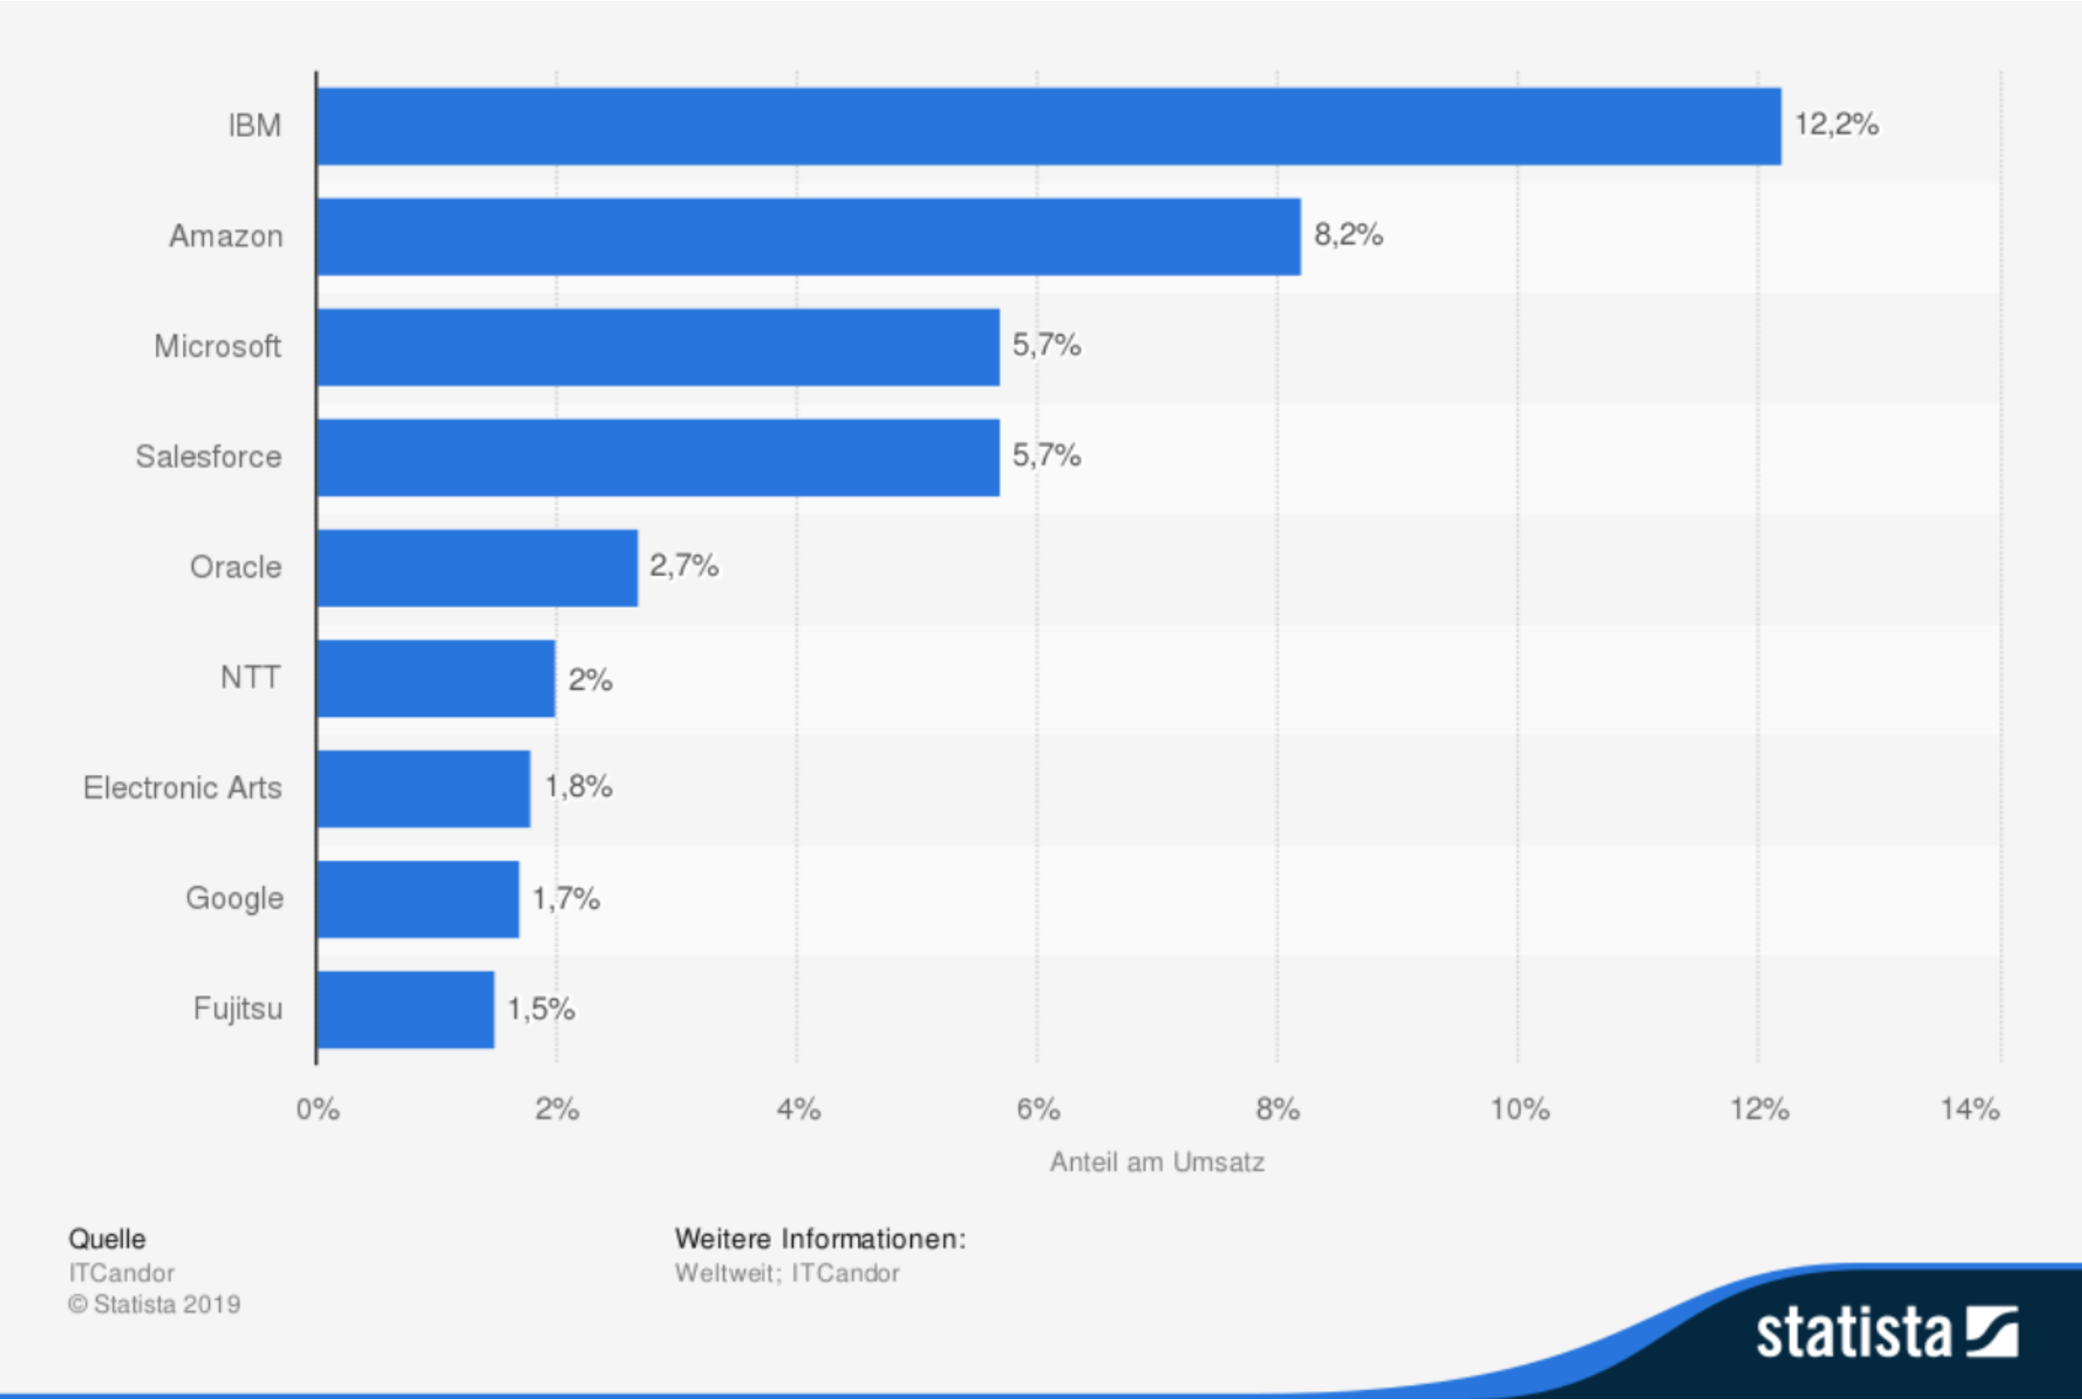
\includegraphics[scale=0.43]{img/statistic_id150979_marktanteile-der-fuehrenden-unternehmen-im-bereich-cloud-computing-weltweit-2019.pdf}
	\caption{Marktanteile der führenden Unternehmen am Umsatz im Bereich Cloud Computing weltweit von Juli 2018 bis Juni 2019}
	{\footnotesize Quelle: \cite{itcandor_cloud_2019}}
	\label{abb:marktanteileCC19}
	%		{\scriptsize \textit{Alle Rechte, einschließlich der Vervielfältigung, Veröffentlichung, Bearbeitung und Übersetzung bleiben der SV Informatik GmbH vorbehalten.}}
\end{figure}

\begin{figure}[H]
	\centering
	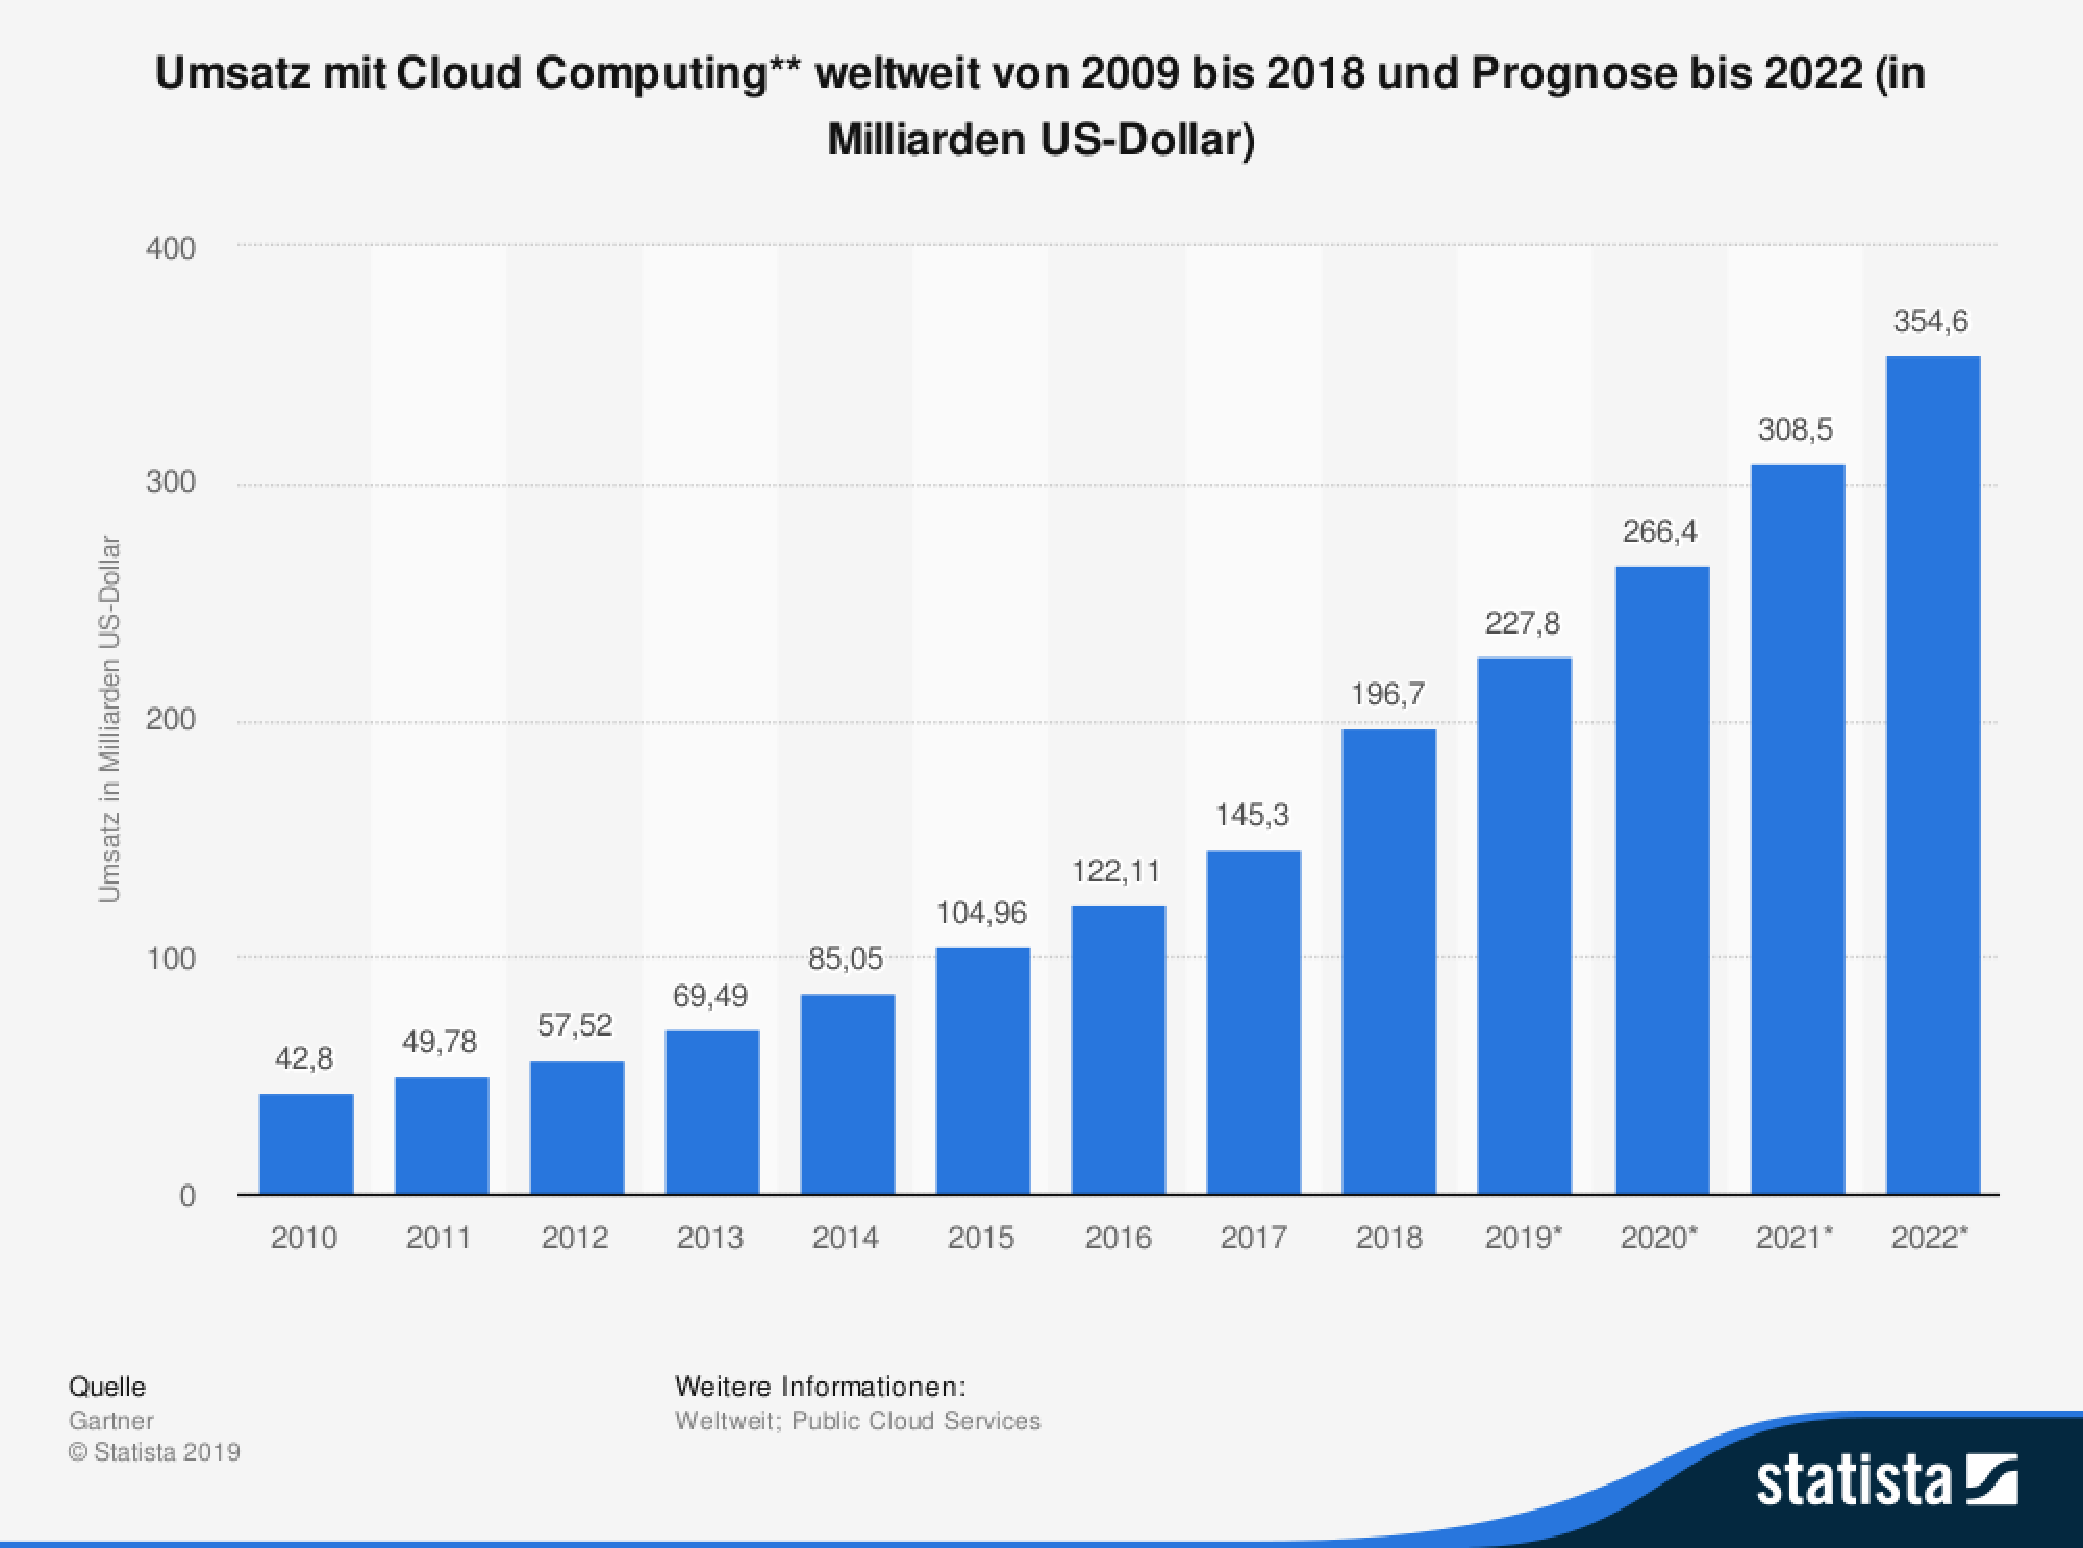
\includegraphics[scale=0.43]{img/statistic_id195760_prognose-zum-umsatz-mit-cloud-computing-weltweit-bis-2022.pdf}
	\caption{Umsatz mit Cloud-Computing weltweit von 2009 bis 2018 und Prognose bis 2022 }
	{\footnotesize Quelle: \cite{gartner_cloud_2019}}
	\label{abb:umsatzprognoseCC}
	%		{\scriptsize \textit{Alle Rechte, einschließlich der Vervielfältigung, Veröffentlichung, Bearbeitung und Übersetzung bleiben der SV Informatik GmbH vorbehalten.}}
\end{figure}

\section{Ergänzungen zum Kapitel Container(-isierung) und Orchestrierung}

\begin{figure}[H]
	\centering
	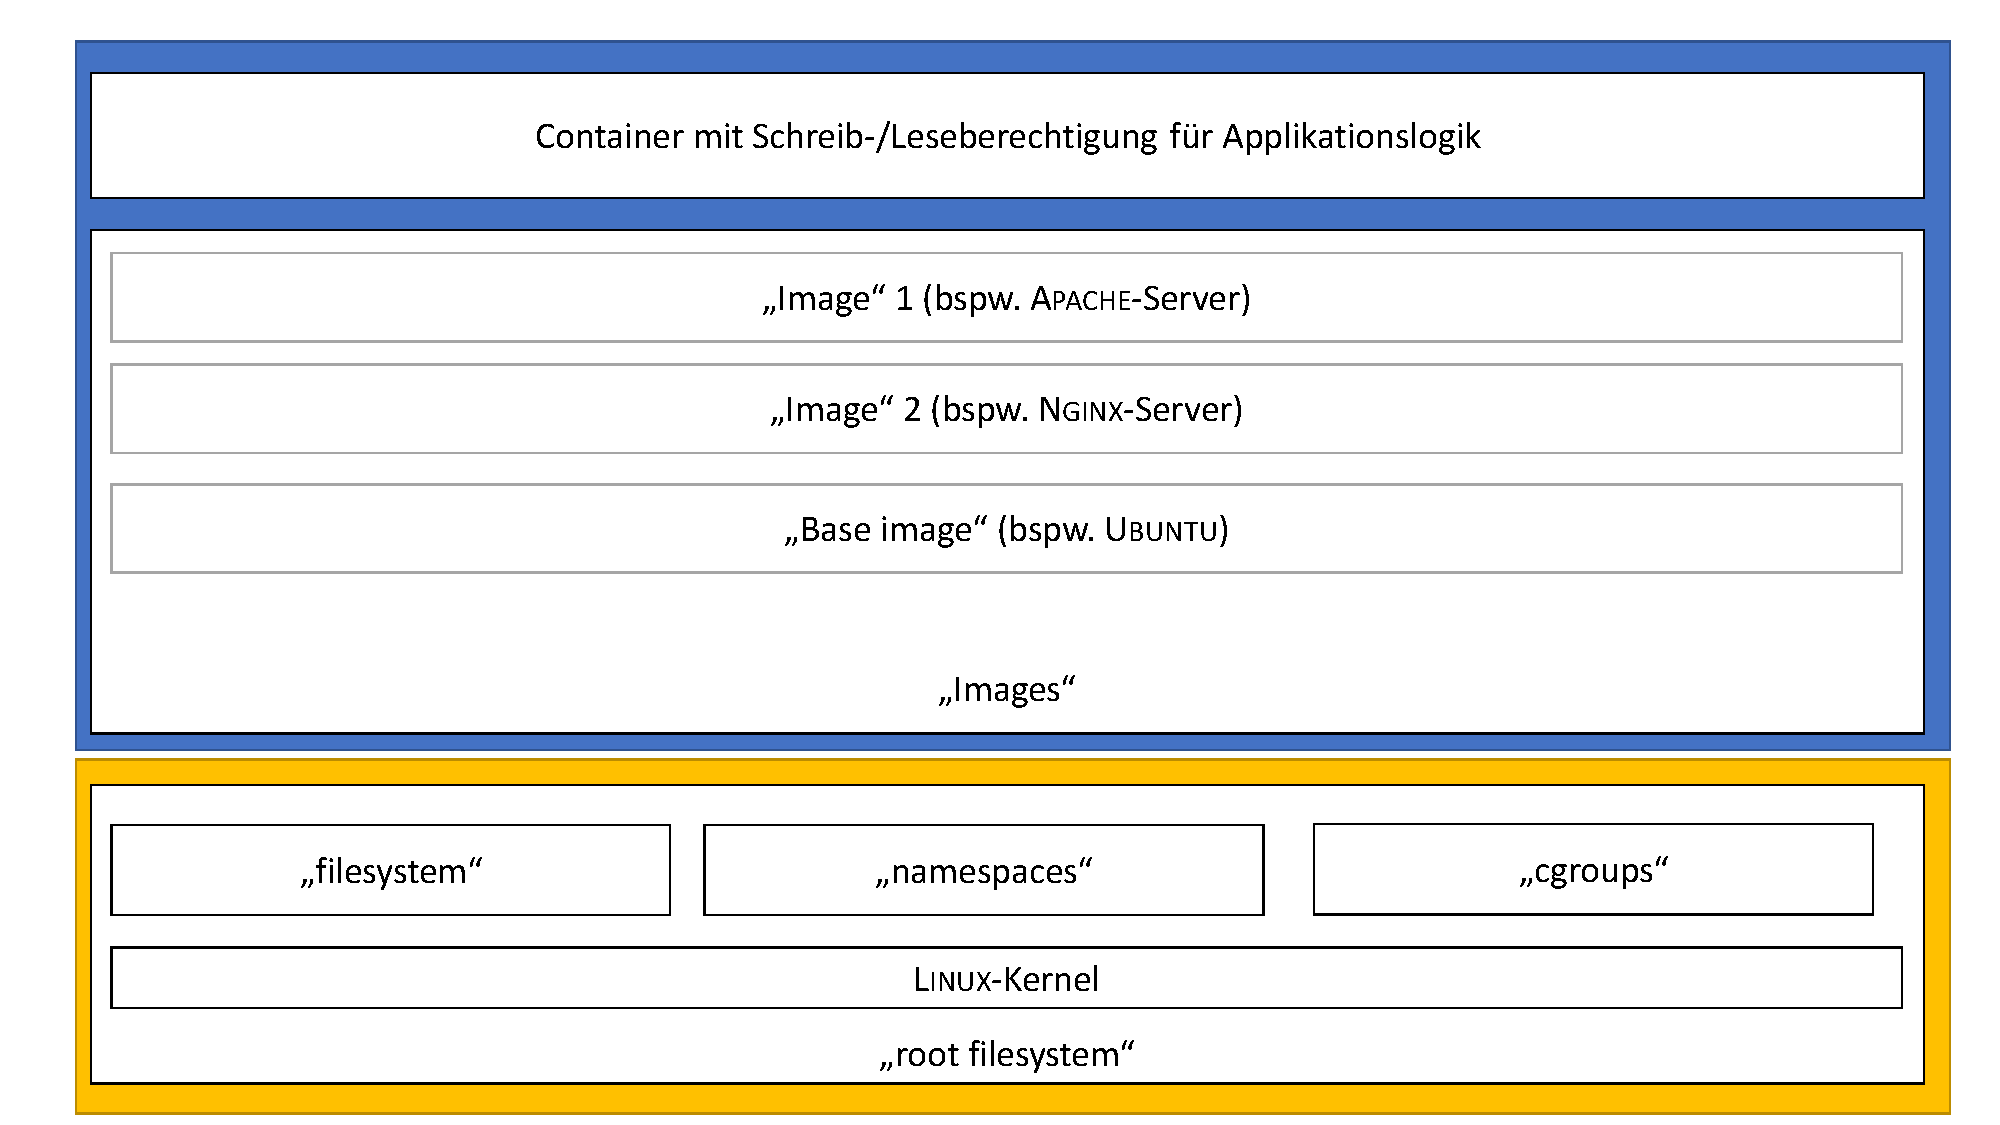
\includegraphics[scale=0.45]{img/containerImageArch.pdf}
	\caption{Architektur des Container-\enquote{Images}}
	{\footnotesize Quelle: in Anlehnung an \cite{pahl_containerization_2015}}
	\label{abb:containerArch}
	%		{\scriptsize \textit{Alle Rechte, einschließlich der Vervielfältigung, Veröffentlichung, Bearbeitung und Übersetzung bleiben der SV Informatik GmbH vorbehalten.}}
\end{figure}

Hierbei ist zu beachten, dass das orange gefärbte die Funktionalitäten der \textsc{Docker}-\enquote{Engine} und das blau gefärbte die möglichen Bestandteile eines \textsc{Docker}-\enquote{Images} darstellen soll.


\begin{figure}[H]
	\centering
	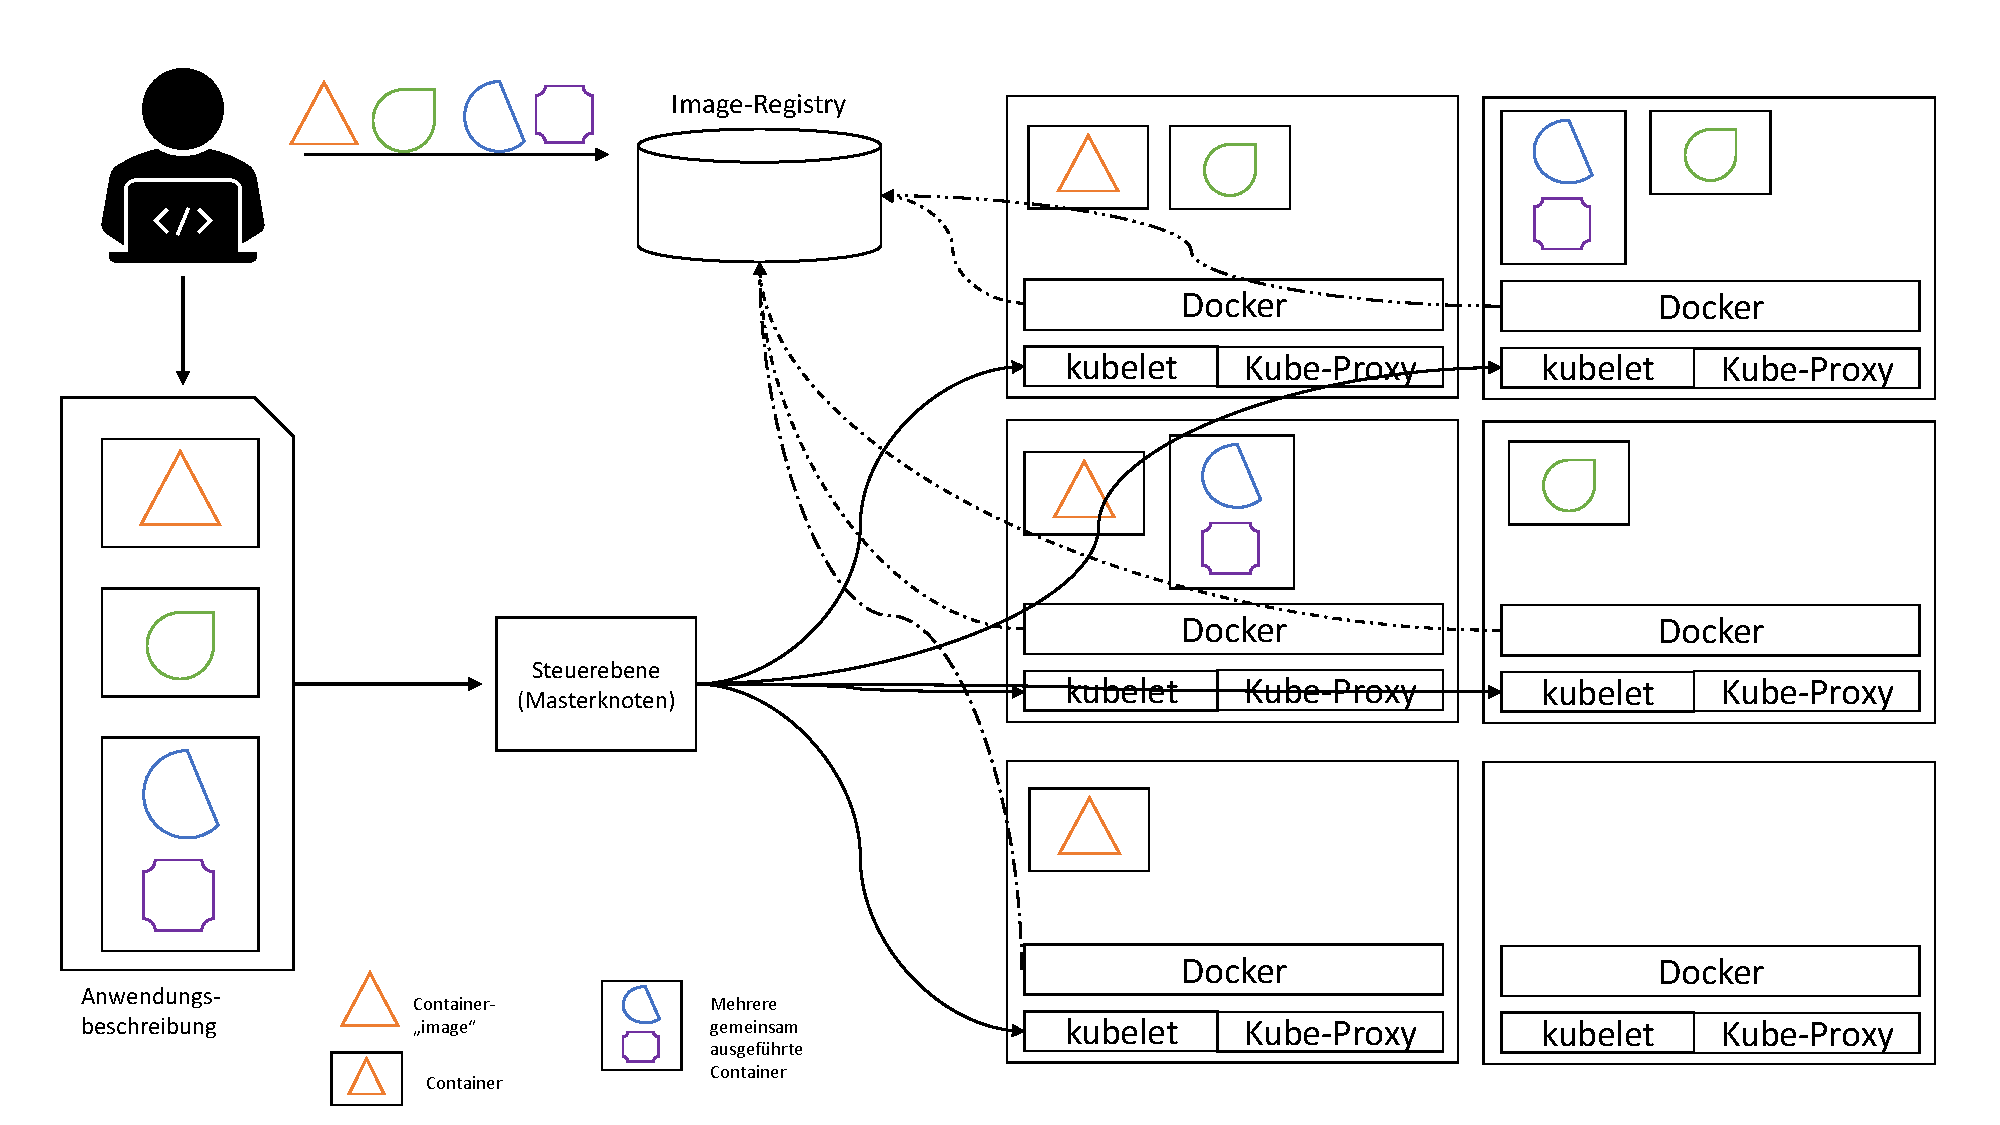
\includegraphics[scale=0.46]{img/k8sArch.pdf}
	\caption{Überblick über eine \textsc{Kubernetes}-Architektur}
	{\footnotesize Quelle: in Anlehnung an \cite[][S.23]{luksa_kubernetes_2018}}
	\label{abb:k8sArch}
	%		{\scriptsize \textit{Alle Rechte, einschließlich der Vervielfältigung, Veröffentlichung, Bearbeitung und Übersetzung bleiben der SV Informatik GmbH vorbehalten.}}
\end{figure}

\begin{figure}[H]
	\centering
	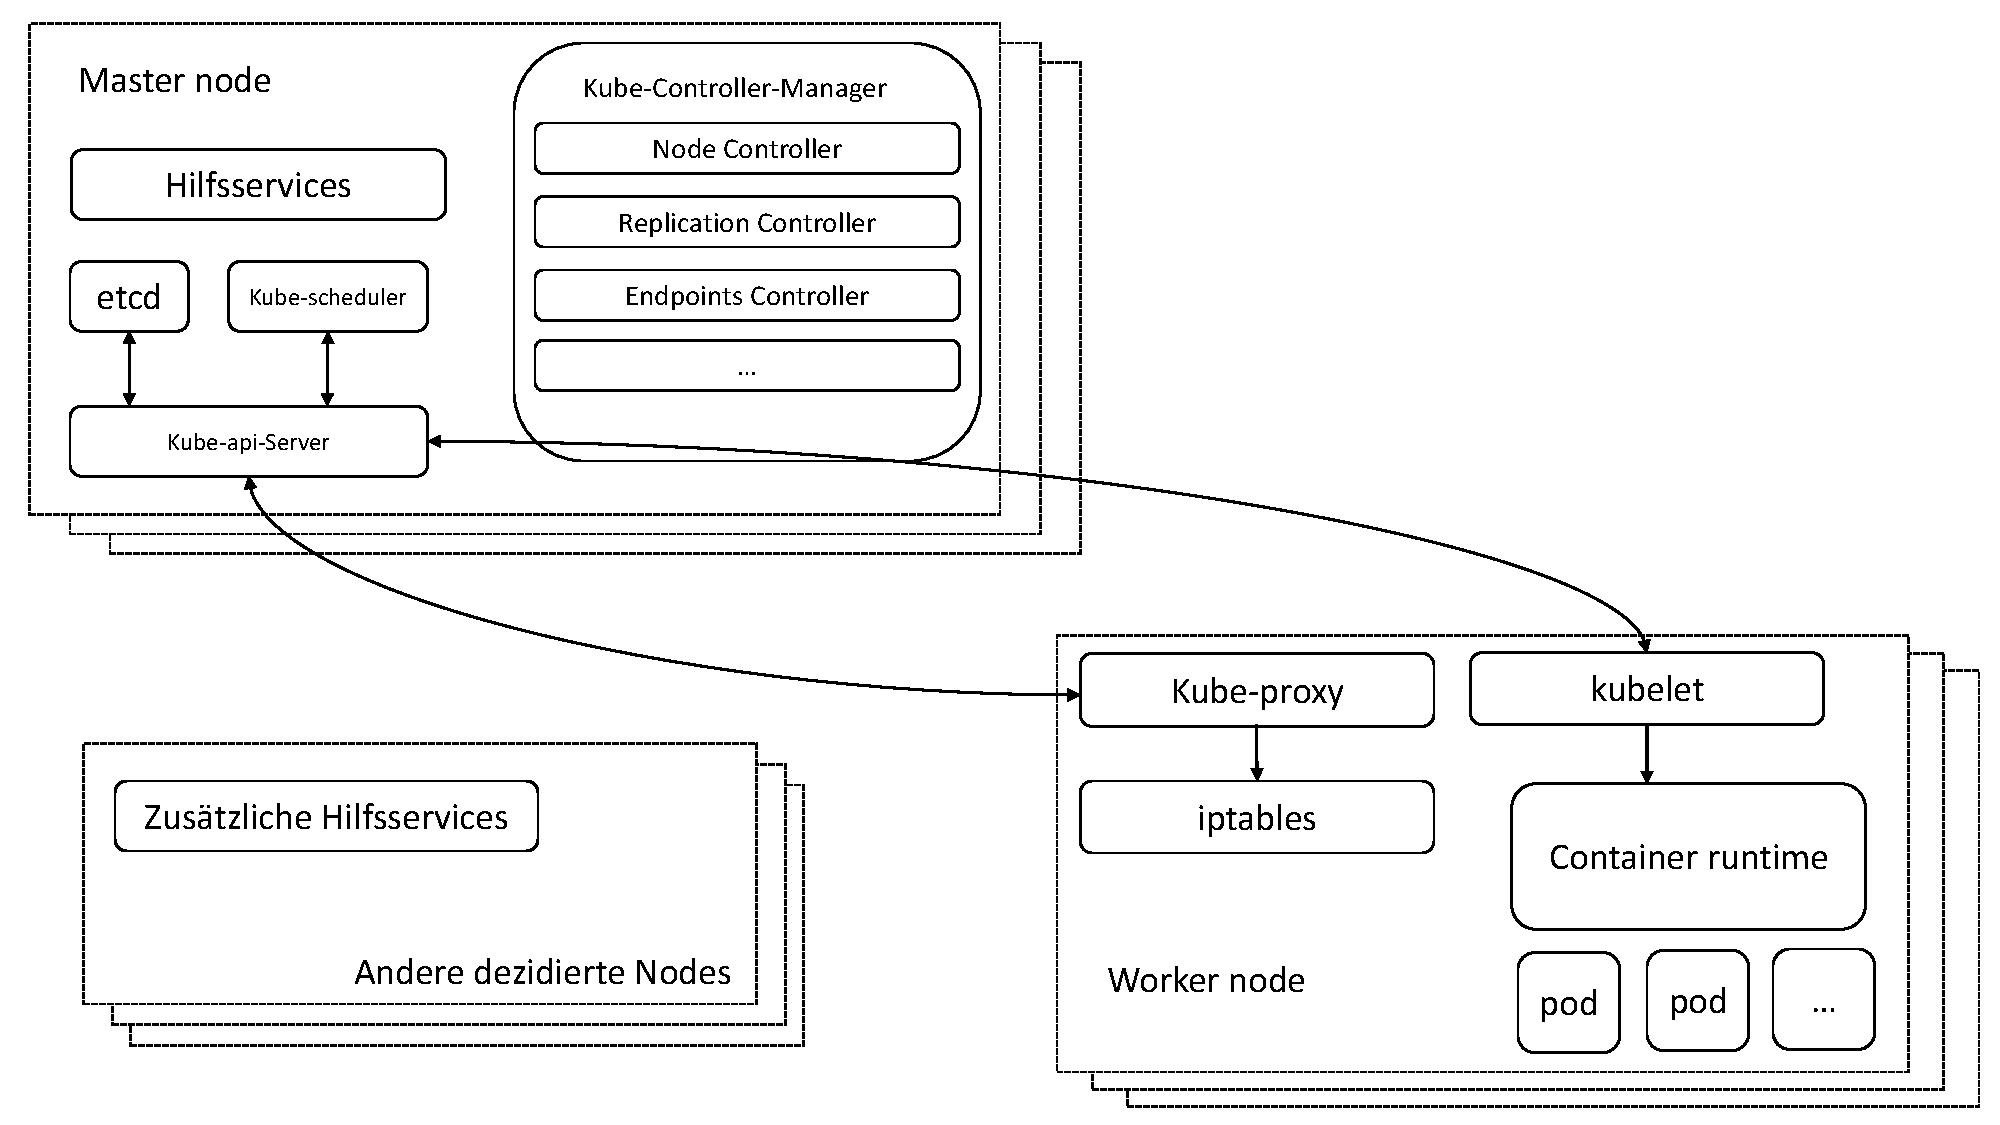
\includegraphics[scale=0.46]{img/k8sArchInteraktion.pdf}
	\caption{Architektur der \enquote{\ac{K8s}}-Interaktion}
	{\footnotesize Quelle: in Anlehnung an \cite[][S.15]{caban_architecting_2019}}
	\label{abb:k8sArchInteraktion}
	%		{\scriptsize \textit{Alle Rechte, einschließlich der Vervielfältigung, Veröffentlichung, Bearbeitung und Übersetzung bleiben der SV Informatik GmbH vorbehalten.}}
\end{figure}

\chapter{Ergänzungen zur Forschungsfrage zwei} \label{appendixFF2}
In diesem Teil des Anhangs sind Ergänzungen zur Forschungsfrage zwei des Kapitels \vref{ff2} beschrieben.

\section{Entscheidung über die Notwendigkeit eines \enquote{Business Case}}

\begin{figure}[H]
	\centering
	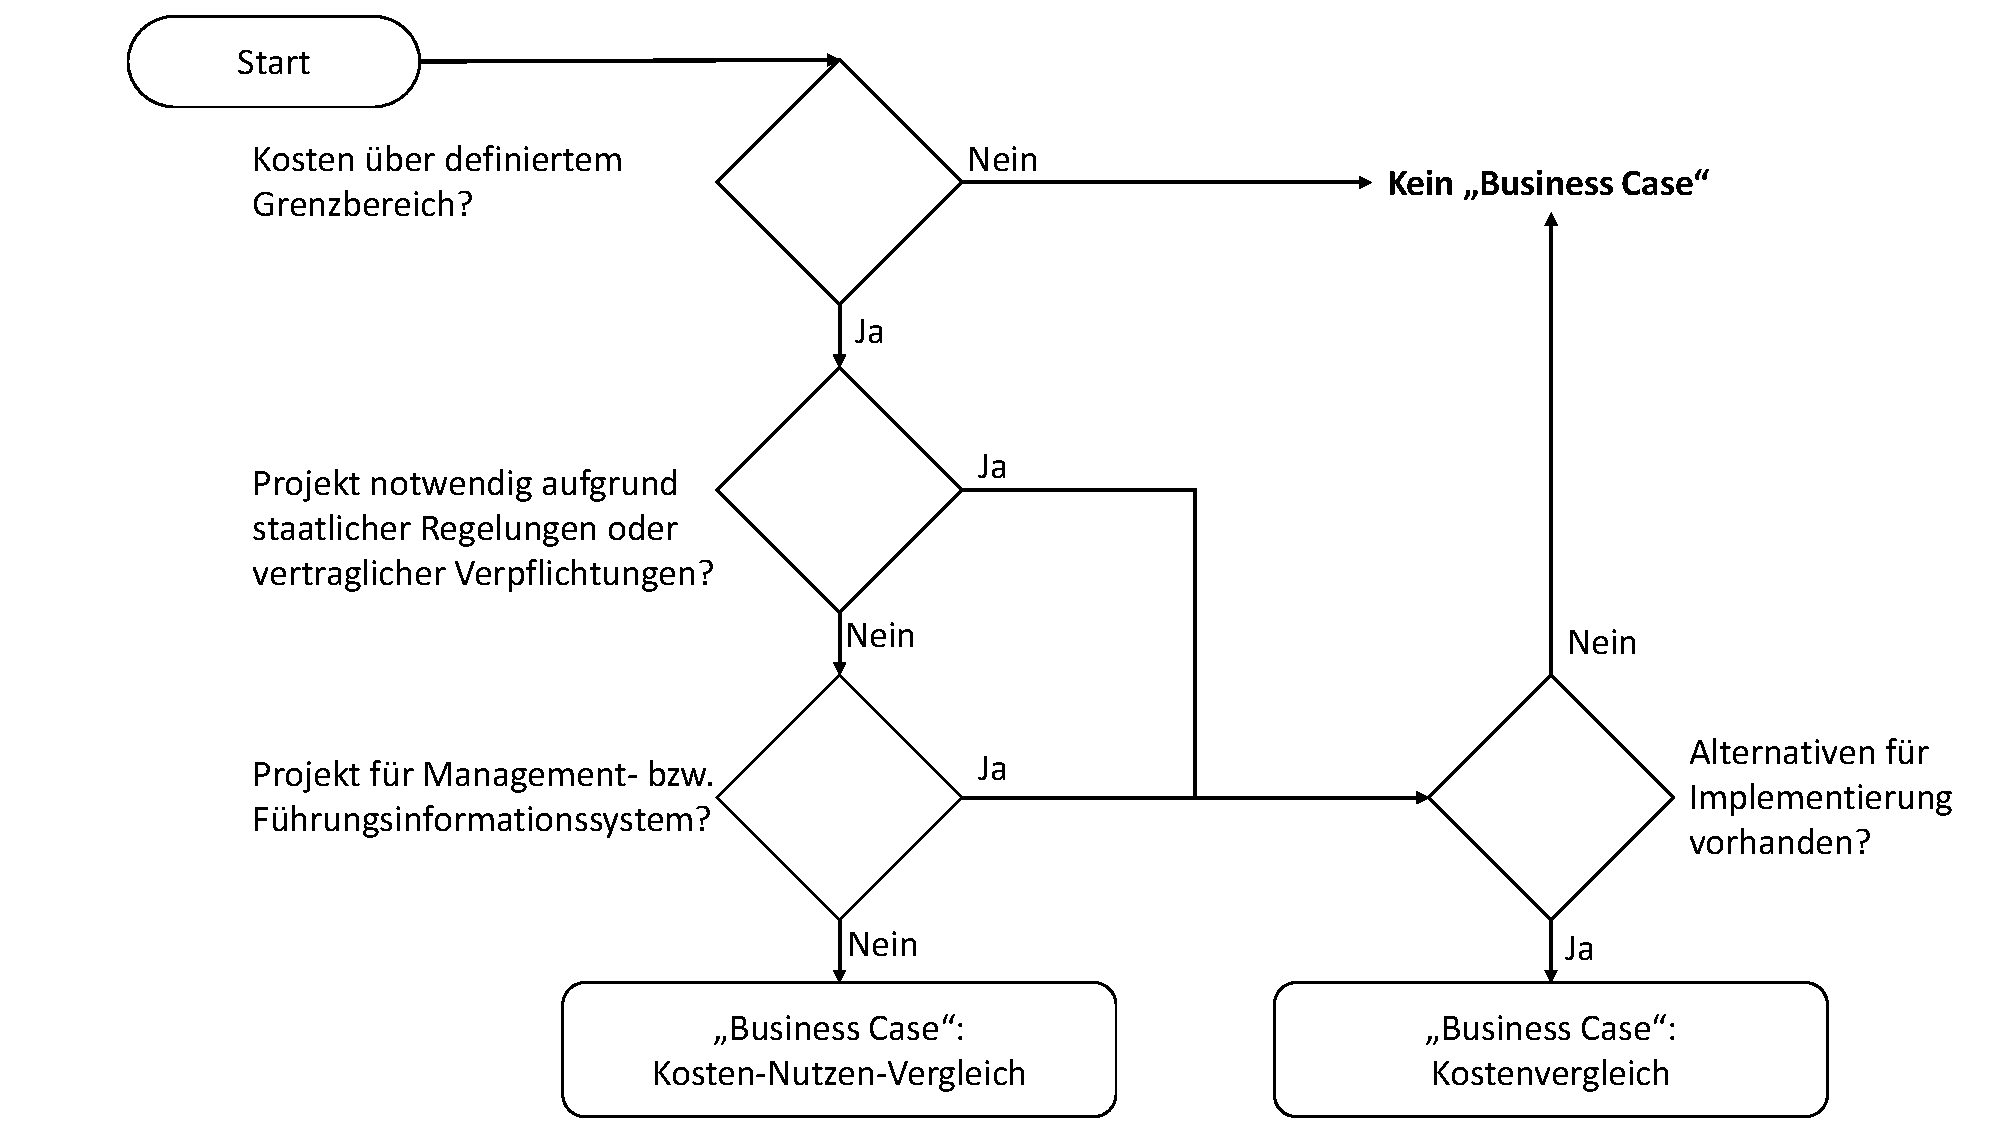
\includegraphics[scale=0.48]{img/entscheidungBC.pdf}
	\caption{Notwendigkeit eines \enquote{Business Case}}
	{\footnotesize Quelle: in Anlehnung an \cite[][S.29]{brugger_it_2009}}
	\label{abb:entscheidungBC}
	%		{\scriptsize \textit{Alle Rechte, einschließlich der Vervielfältigung, Veröffentlichung, Bearbeitung und Übersetzung bleiben der SV Informatik GmbH vorbehalten.}}
\end{figure}

\section{Vor-/Nachteile der internen beziehungsweise externen Erstellung eines \enquote{Business Case}}\label{appendixVorNachteileErstellungBC}

\begin{table*}[h!]
	\centering
	\ra{1.3} %more space beetween rules
	
	\begin{tabular}{@{}ll@{}}\toprule[1.5pt]
		
		\textbf{Vorteile} & \textbf{Nachteile} \\ \midrule
		
		% below rules with content
		Neutralität & Kein Wissenstransfer \\
		Verfügbarkeit & Kosten, egal ob der \enquote{Business Case} rentabel ist\\
		Effiziente Erstellung & hohe Kosten im Vergleich zur internen Erstellung \\
		Glaubwürdigkeit & Abhängigkeit \\
		Qualität & Verlust der firmeninternen Standards \\
		Innovation & \\
		Schlichtung & \\
		
		\bottomrule[1.5pt]
	\end{tabular}
	
	\caption{Überblick über die Vor-/Nachteile der externen Erstellung eines \enquote{Business Case}}
	{\footnotesize Quelle: in Anlehnung an \cite[][S.34]{brugger_it_2009}}
	\label{tab:externVorNachteile}
	
\end{table*}

\begin{table*}[h!]
	\centering
	\ra{1.3} %more space beetween rules
	
	\begin{tabular}{@{}ll@{}}\toprule[1.5pt]
		
		\textbf{Vorteile} & \textbf{Nachteile} \\ \midrule
		
		% below rules with content
		Wissensaufbau & Verfügbarkeit \\
		Qualität & Effizienzverlust bei rein technischen/operativen Mitarbeitern \\
		\enquote{Teamwork} & Glaubwürdigkeit \\
		Standardisierung & Qualitätskontrolle durch \enquote{Controlling}-Division \\
		
		\bottomrule[1.5pt]
	\end{tabular}
	
	\caption{Überblick über die Vor-/Nachteile der internen Erstellung eines \enquote{Business Case}}
	{\footnotesize Quelle: in Anlehnung an \cite[][S.34]{brugger_it_2009}}
	\label{tab:internVorNachteile}
	
\end{table*}

\begin{figure}[H]
	\centering
	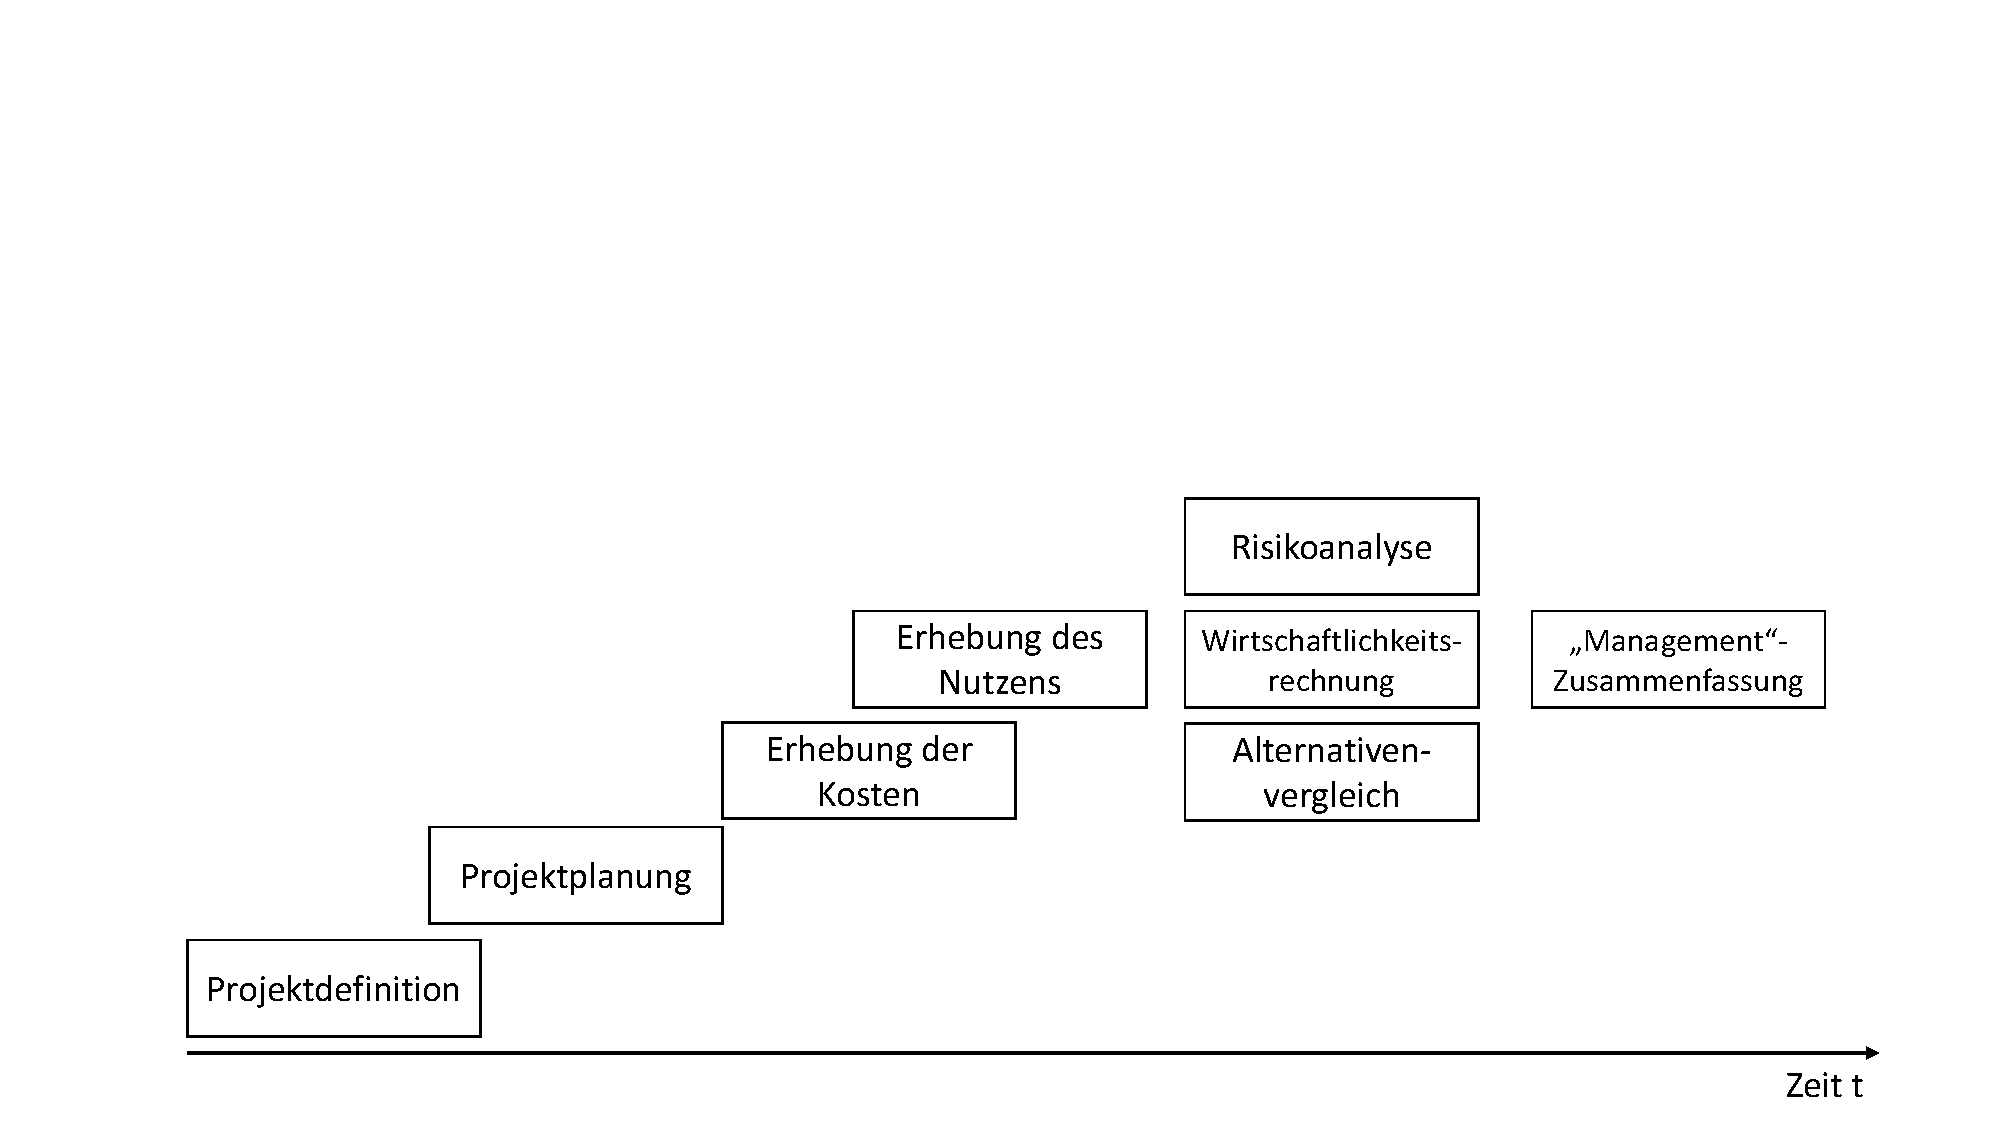
\includegraphics[scale=0.48]{img/chronoBC.pdf}
	\caption{Chronologische Abfolge der Entwicklungsphase eines \enquote{Business Case}}
	{\footnotesize Quelle: in Anlehnung an \cite[][]{herman_is_2009}}
	\label{abb:entwicklungBC}
	%		{\scriptsize \textit{Alle Rechte, einschließlich der Vervielfältigung, Veröffentlichung, Bearbeitung und Übersetzung bleiben der SV Informatik GmbH vorbehalten.}}
\end{figure}

\chapter{Ergänzungen zur Forschungsfrage drei} \label{appendixFF3}
In diesem Teil des Anhangs sind Ergänzungen zur Forschungsfrage drei des Kapitels \vref{ff3} beschrieben.

\section{\enquote{Plan-Do-Check-Act}-Regelkreis}

\begin{figure}[H]
	\centering
	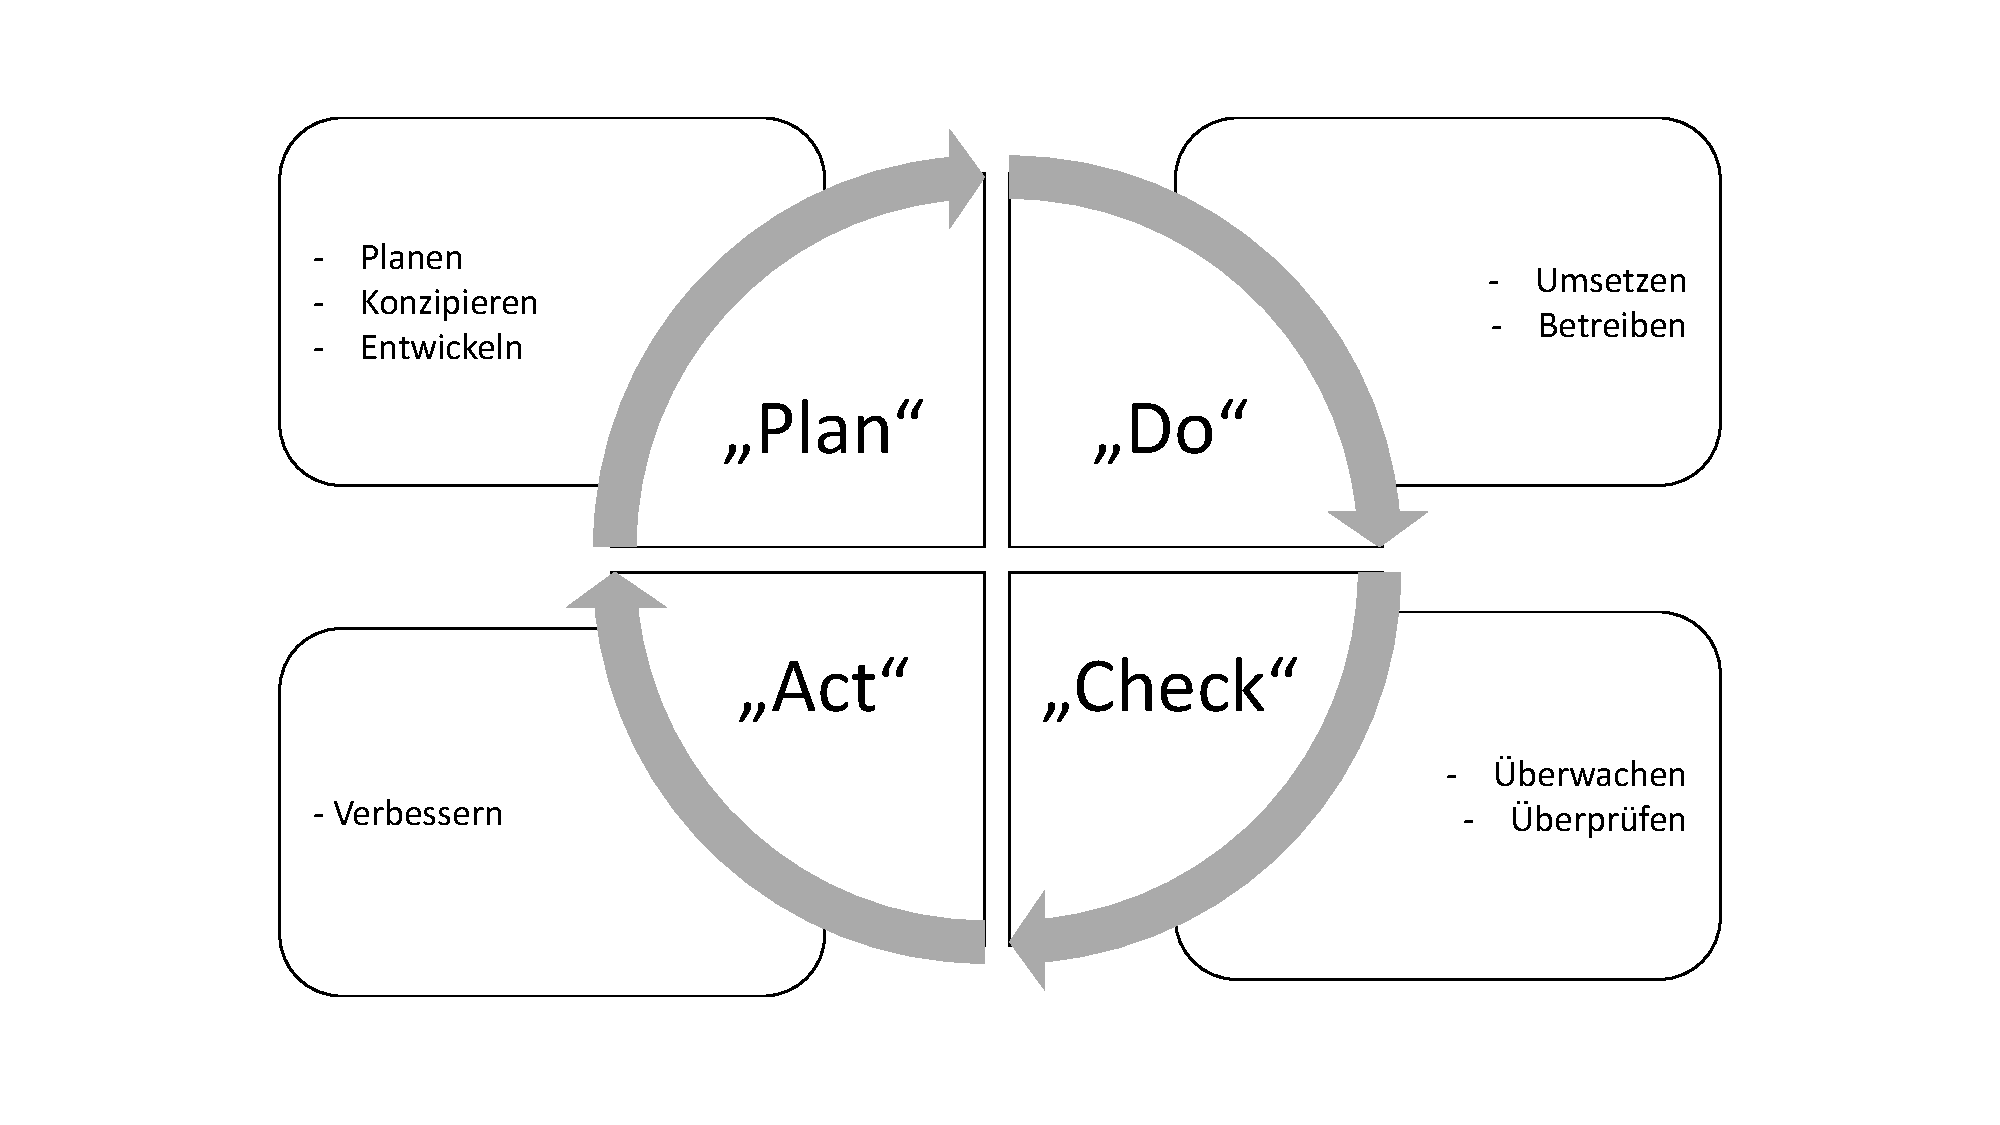
\includegraphics[scale=0.51]{img/planDoCheckAct.pdf}
	\caption{Der \enquote{Plan-Do-Check-Act}-Regelkreis}
	{\footnotesize Quelle: in Anlehnung an \cite[][S.12]{kersten_it-sicherheitsmanagement_2020}}
	\label{abb:planDoCheckAct}
	%		{\scriptsize \textit{Alle Rechte, einschließlich der Vervielfältigung, Veröffentlichung, Bearbeitung und Übersetzung bleiben der SV Informatik GmbH vorbehalten.}}
\end{figure}

\clearpage % neue Seite
\section{Checkliste zur Vorbereitung der \ac{ISMS}-Einführung}
\begin{table*}[h!]
	\centering
	\ra{1.3} %more space beetween rules
	
	\begin{tabular}{@{}lp{10cm}l@{}}\toprule[1.5pt]
		
		\textbf{Aktion} & \textbf{Gegenstand} & \textbf{Erfüllt?} \\ \midrule
		% below rules with content
		
		1 & Sind die Normen (27000, 27001, 27002) in aktueller elektronischer
		Form vorhanden? & $\square$ \\
		2 & Sind die Vorteile und der Nutzen eines ISMS erläutert worden? & $\square$ \\
		3 & Ist ein Grob-Abgleich mit ISO 27001 erfolgt? (Ziel: erste
		Aufwandsabschätzung) & $\square$ \\
		4 & Ist eine Entscheidung zur Orientierung an der ISO 27001
		getroffen worden? & $\square$ \\
		5 & Denken wir in Management-Systemen? Existieren schon andere
		Management-Systeme? & $\square$ \\
		6 & Ist der Begriff ISMS eingeführt? & $\square$ \\
		7 & Denken wir in Geschäftsprozessen und informationstechnischen Anwendungen? & $\square$ \\
		8 & Ist der Anwendungsbereich des ISMS (Scope) zumindest grob
		skizziert? & $\square$ \\
		9 & Sind zumindest die Top Level Assets und deren Asset/Risk
		Owner erfasst worden? & $\square$ \\
		10 & Wurden – zumindest grob – Sicherheitsziele für diese Assets
		festgelegt? & $\square$ \\
				
		\bottomrule[1.5pt]
	\end{tabular}
	
	\caption{Checkliste zur Vorbereitung der \ac{ISMS}-Einführung}
	{\footnotesize{Quelle: in Anlehnung an \cite[][S.15]{kersten_it-sicherheitsmanagement_2020}}}
	\label{tab:checklisteVorbereitungISMS}
	
\end{table*}

\clearpage
\section{Schichtenmodell des IT-Grundschutzes}
\begin{figure}[H]
	\centering
	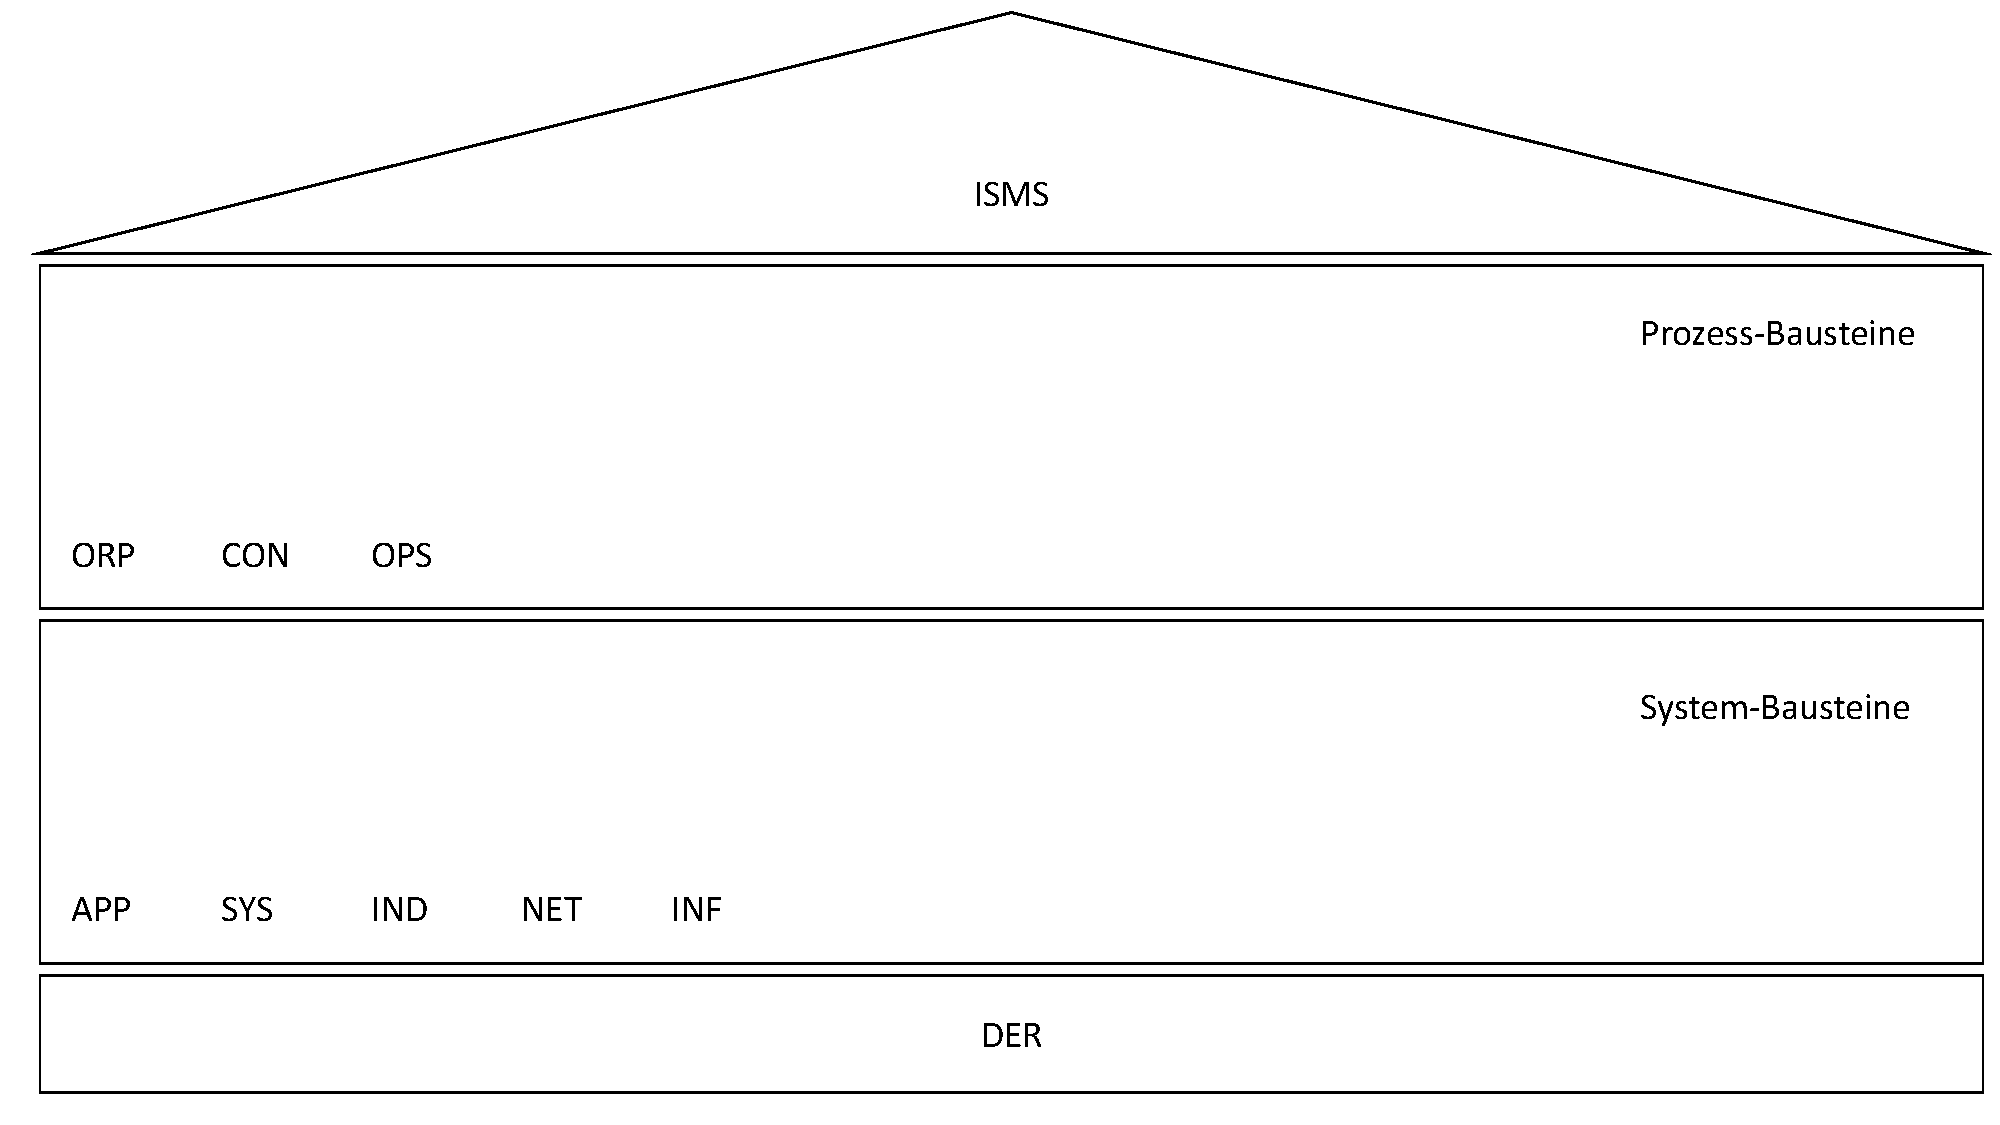
\includegraphics[scale=0.45]{img/bsiSchichtenmodell.pdf}
	\caption{Das Schichtenmodell des IT-Grundschutzes}
	{\footnotesize Quelle: in Anlehnung an \cite[][S.9]{bundesamt_fur_sicherheit_in_der_informationstechnik_bsi_it-grundschutz-kompendium_2020}}
	\label{abb:BSISchichtenmodell}
	%		{\scriptsize \textit{Alle Rechte, einschließlich der Vervielfältigung, Veröffentlichung, Bearbeitung und Übersetzung bleiben der SV Informatik GmbH vorbehalten.}}
\end{figure}

\enquote{Die Prozessbausteine, die in der Regel für sämtliche oder große Teile eines Informationsverbunds gleichermaßen
gelten, unterteilen sich in die folgenden Schichten, die wiederum aus weiteren Teilschichten bestehen können.
\begin{itemize}
	\item Die Schicht ISMS enthält als Grundlage für alle weiteren Aktivitäten im Sicherheitsprozess den Baustein Sicherheitsmanagement.
	\item Die Schicht ORP befasst sich mit organisatorischen und personellen Sicherheitsaspekten. In diese Schicht fallen beispielsweise die Bausteine Organisation und Personal.
	\item Die Schicht CON enthält Bausteine, die sich mit Konzepten und Vorgehensweisen befassen. Typische Bausteine
	der Schicht CON sind unter anderem Kryptokonzept und Datenschutz.
	\item Die Schicht OPS umfasst alle Sicherheitsaspekte betrieblicher Art. Insbesondere sind dies die Sicherheitsaspekte des operativen IT-Betriebs, sowohl bei einem Betrieb im Haus, als auch bei einem IT-Betrieb, der in Teilen oder komplett durch Dritte betrieben wird. Ebenso enthält er die Sicherheitsaspekte, die bei einem IT-Betrieb für Dritte zu beachten sind. Beispiele für die Schicht OPS sind die Bausteine Schutz vor Schadprogrammen und Outsourcing für Kunden.
	\item In der Schicht DER finden sich alle Bausteine, die für die Überprüfung der umgesetzten Sicherheitsmaßnahmen, die Detektion von Sicherheitsvorfällen sowie die geeigneten Reaktionen darauf relevant sind. Typische Bausteine der Schicht DER sind Behandlung von Sicherheitsvorfällen und Vorsorge für IT-Forensik.
\end{itemize}
Neben den Prozess-Bausteinen beinhaltet das IT-Grundschutz-Kompendium auch System-Bausteine. Diese werden
in der Regel auf einzelne Zielobjekte oder Gruppen von Zielobjekten angewendet. Die System-Bausteine unterteilen sich in die folgenden Schichten. Ähnlich wie die Prozess-Bausteine können auch die System-Bausteine aus weiteren Teilschichten bestehen.

\begin{itemize}
	\item Die Schicht APP beschäftigt sich mit der Absicherung von Anwendungen und Diensten, unter anderem in den
	Bereichen Kommunikation, Verzeichnisdienste, netzbasierte Dienste sowie Business- und Client-Anwendungen.
	Typische Bausteine der Schicht APP sind Allgemeine Groupware, Office-Produkte, Webserver und Relationale
	Datenbanksysteme.
	\item Die Schicht SYS betrifft die einzelnen IT-Systeme des Informationsverbunds, die ggf. in Gruppen zusammengefasst wurden. Hier werden die Sicherheitsaspekte von Servern, Desktop-Systemen, Mobile Devices und sonstigen IT-Systemen wie Druckern und TK-Anlagen behandelt. Zur Schicht SYS gehören beispielsweise Bausteine zu
	konkreten Betriebssystemen, Allgemeine Smartphones und Tablets sowie Drucker, Kopierer und Multifunktionsgeräte.
	\item Die Schicht IND befasst sich mit Sicherheitsaspekten industrieller IT. In diese Schicht fallen beispielsweise die Bausteine Betriebs- und Steuerungstechnik, Allgemeine ICS-Komponente und Speicherprogrammierbare Steuerung (SPS).
	\item Die Schicht NET betrachtet die Vernetzungsaspekte, die sich nicht primär auf bestimmte IT-Systeme, sondern
	auf die Netzverbindungen und die Kommunikation beziehen. Dazu gehören zum Beispiel die Bausteine NetzManagement, Firewall und WLAN-Betrieb.
	\item Die Schicht INF befasst sich mit den baulich-technischen Gegebenheiten, hier werden Aspekte der infrastrukturellen Sicherheit zusammengeführt. Dies betrifft unter anderem die Bausteine Allgemeines Gebäude und Rechenzentrum.
\end{itemize}}\autocite[][S.23-24]{bundesamt_fur_sicherheit_in_der_informationstechnik_bsi_it-grundschutz-kompendium_2020}




% Ehrenwörtliche Erklärung ewerkl.tex einziehen
% !TEX root =  master.tex

\clearpage
\chapter*{Ehrenwörtliche Erklärung}

% Wird die folgende Zeile auskommentiert, erscheint die ehrenwörtliche
% Erklärung im Inhaltsverzeichnis.
\addcontentsline{toc}{chapter}{Ehrenwörtliche Erklärung}

Ich versichere hiermit, dass ich die vorliegende Arbeit mit dem Thema: \textit{\DerTitelDerArbeit} selbstständig verfasst und keine anderen als die angegebenen Quellen und Hilfsmittel benutzt habe. Ich versichere zudem, dass die eingereichte elektronische Fassung mit der gedruckten Fassung übereinstimmt.

%\vspace{3cm}
%\noindent\rule{5cm}{.4pt}\hfill\rule{5cm}{.4pt}\par
%Ort, Datum \hfill \DerAutorDerArbeit

\vspace{3cm}
\noindent Mannheim, 08.05.2020 \hfill\rule{5cm}{.4pt}\par
\noindent\hfill \DerAutorDerArbeit



\end{document}
